% Options for packages loaded elsewhere
% Options for packages loaded elsewhere
\PassOptionsToPackage{unicode}{hyperref}
\PassOptionsToPackage{hyphens}{url}
\PassOptionsToPackage{dvipsnames,svgnames,x11names}{xcolor}
%
\documentclass[
  11pt,
]{article}
\usepackage{xcolor}
\usepackage[margin=1in]{geometry}
\usepackage{amsmath,amssymb}
\setcounter{secnumdepth}{5}
\usepackage{iftex}
\ifPDFTeX
  \usepackage[T1]{fontenc}
  \usepackage[utf8]{inputenc}
  \usepackage{textcomp} % provide euro and other symbols
\else % if luatex or xetex
  \usepackage{unicode-math} % this also loads fontspec
  \defaultfontfeatures{Scale=MatchLowercase}
  \defaultfontfeatures[\rmfamily]{Ligatures=TeX,Scale=1}
\fi
\usepackage{lmodern}
\ifPDFTeX\else
  % xetex/luatex font selection
\fi
% Use upquote if available, for straight quotes in verbatim environments
\IfFileExists{upquote.sty}{\usepackage{upquote}}{}
\IfFileExists{microtype.sty}{% use microtype if available
  \usepackage[]{microtype}
  \UseMicrotypeSet[protrusion]{basicmath} % disable protrusion for tt fonts
}{}
\makeatletter
\@ifundefined{KOMAClassName}{% if non-KOMA class
  \IfFileExists{parskip.sty}{%
    \usepackage{parskip}
  }{% else
    \setlength{\parindent}{0pt}
    \setlength{\parskip}{6pt plus 2pt minus 1pt}}
}{% if KOMA class
  \KOMAoptions{parskip=half}}
\makeatother
% Make \paragraph and \subparagraph free-standing
\makeatletter
\ifx\paragraph\undefined\else
  \let\oldparagraph\paragraph
  \renewcommand{\paragraph}{
    \@ifstar
      \xxxParagraphStar
      \xxxParagraphNoStar
  }
  \newcommand{\xxxParagraphStar}[1]{\oldparagraph*{#1}\mbox{}}
  \newcommand{\xxxParagraphNoStar}[1]{\oldparagraph{#1}\mbox{}}
\fi
\ifx\subparagraph\undefined\else
  \let\oldsubparagraph\subparagraph
  \renewcommand{\subparagraph}{
    \@ifstar
      \xxxSubParagraphStar
      \xxxSubParagraphNoStar
  }
  \newcommand{\xxxSubParagraphStar}[1]{\oldsubparagraph*{#1}\mbox{}}
  \newcommand{\xxxSubParagraphNoStar}[1]{\oldsubparagraph{#1}\mbox{}}
\fi
\makeatother

\usepackage{color}
\usepackage{fancyvrb}
\newcommand{\VerbBar}{|}
\newcommand{\VERB}{\Verb[commandchars=\\\{\}]}
\DefineVerbatimEnvironment{Highlighting}{Verbatim}{commandchars=\\\{\}}
% Add ',fontsize=\small' for more characters per line
\usepackage{framed}
\definecolor{shadecolor}{RGB}{241,243,245}
\newenvironment{Shaded}{\begin{snugshade}}{\end{snugshade}}
\newcommand{\AlertTok}[1]{\textcolor[rgb]{0.68,0.00,0.00}{#1}}
\newcommand{\AnnotationTok}[1]{\textcolor[rgb]{0.37,0.37,0.37}{#1}}
\newcommand{\AttributeTok}[1]{\textcolor[rgb]{0.40,0.45,0.13}{#1}}
\newcommand{\BaseNTok}[1]{\textcolor[rgb]{0.68,0.00,0.00}{#1}}
\newcommand{\BuiltInTok}[1]{\textcolor[rgb]{0.00,0.23,0.31}{#1}}
\newcommand{\CharTok}[1]{\textcolor[rgb]{0.13,0.47,0.30}{#1}}
\newcommand{\CommentTok}[1]{\textcolor[rgb]{0.37,0.37,0.37}{#1}}
\newcommand{\CommentVarTok}[1]{\textcolor[rgb]{0.37,0.37,0.37}{\textit{#1}}}
\newcommand{\ConstantTok}[1]{\textcolor[rgb]{0.56,0.35,0.01}{#1}}
\newcommand{\ControlFlowTok}[1]{\textcolor[rgb]{0.00,0.23,0.31}{\textbf{#1}}}
\newcommand{\DataTypeTok}[1]{\textcolor[rgb]{0.68,0.00,0.00}{#1}}
\newcommand{\DecValTok}[1]{\textcolor[rgb]{0.68,0.00,0.00}{#1}}
\newcommand{\DocumentationTok}[1]{\textcolor[rgb]{0.37,0.37,0.37}{\textit{#1}}}
\newcommand{\ErrorTok}[1]{\textcolor[rgb]{0.68,0.00,0.00}{#1}}
\newcommand{\ExtensionTok}[1]{\textcolor[rgb]{0.00,0.23,0.31}{#1}}
\newcommand{\FloatTok}[1]{\textcolor[rgb]{0.68,0.00,0.00}{#1}}
\newcommand{\FunctionTok}[1]{\textcolor[rgb]{0.28,0.35,0.67}{#1}}
\newcommand{\ImportTok}[1]{\textcolor[rgb]{0.00,0.46,0.62}{#1}}
\newcommand{\InformationTok}[1]{\textcolor[rgb]{0.37,0.37,0.37}{#1}}
\newcommand{\KeywordTok}[1]{\textcolor[rgb]{0.00,0.23,0.31}{\textbf{#1}}}
\newcommand{\NormalTok}[1]{\textcolor[rgb]{0.00,0.23,0.31}{#1}}
\newcommand{\OperatorTok}[1]{\textcolor[rgb]{0.37,0.37,0.37}{#1}}
\newcommand{\OtherTok}[1]{\textcolor[rgb]{0.00,0.23,0.31}{#1}}
\newcommand{\PreprocessorTok}[1]{\textcolor[rgb]{0.68,0.00,0.00}{#1}}
\newcommand{\RegionMarkerTok}[1]{\textcolor[rgb]{0.00,0.23,0.31}{#1}}
\newcommand{\SpecialCharTok}[1]{\textcolor[rgb]{0.37,0.37,0.37}{#1}}
\newcommand{\SpecialStringTok}[1]{\textcolor[rgb]{0.13,0.47,0.30}{#1}}
\newcommand{\StringTok}[1]{\textcolor[rgb]{0.13,0.47,0.30}{#1}}
\newcommand{\VariableTok}[1]{\textcolor[rgb]{0.07,0.07,0.07}{#1}}
\newcommand{\VerbatimStringTok}[1]{\textcolor[rgb]{0.13,0.47,0.30}{#1}}
\newcommand{\WarningTok}[1]{\textcolor[rgb]{0.37,0.37,0.37}{\textit{#1}}}

\usepackage{longtable,booktabs,array}
\newcounter{none} % for unnumbered tables
\usepackage{calc} % for calculating minipage widths
% Correct order of tables after \paragraph or \subparagraph
\usepackage{etoolbox}
\makeatletter
\patchcmd\longtable{\par}{\if@noskipsec\mbox{}\fi\par}{}{}
\makeatother
% Allow footnotes in longtable head/foot
\IfFileExists{footnotehyper.sty}{\usepackage{footnotehyper}}{\usepackage{footnote}}
\makesavenoteenv{longtable}
\usepackage{graphicx}
\makeatletter
\newsavebox\pandoc@box
\newcommand*\pandocbounded[1]{% scales image to fit in text height/width
  \sbox\pandoc@box{#1}%
  \Gscale@div\@tempa{\textheight}{\dimexpr\ht\pandoc@box+\dp\pandoc@box\relax}%
  \Gscale@div\@tempb{\linewidth}{\wd\pandoc@box}%
  \ifdim\@tempb\p@<\@tempa\p@\let\@tempa\@tempb\fi% select the smaller of both
  \ifdim\@tempa\p@<\p@\scalebox{\@tempa}{\usebox\pandoc@box}%
  \else\usebox{\pandoc@box}%
  \fi%
}
% Set default figure placement to htbp
\def\fps@figure{htbp}
\makeatother


% definitions for citeproc citations
\NewDocumentCommand\citeproctext{}{}
\NewDocumentCommand\citeproc{mm}{%
  \begingroup\def\citeproctext{#2}\cite{#1}\endgroup}
\makeatletter
 % allow citations to break across lines
 \let\@cite@ofmt\@firstofone
 % avoid brackets around text for \cite:
 \def\@biblabel#1{}
 \def\@cite#1#2{{#1\if@tempswa , #2\fi}}
\makeatother
\newlength{\cslhangindent}
\setlength{\cslhangindent}{1.5em}
\newlength{\csllabelwidth}
\setlength{\csllabelwidth}{3em}
\newenvironment{CSLReferences}[2] % #1 hanging-indent, #2 entry-spacing
 {\begin{list}{}{%
  \setlength{\itemindent}{0pt}
  \setlength{\leftmargin}{0pt}
  \setlength{\parsep}{0pt}
  % turn on hanging indent if param 1 is 1
  \ifodd #1
   \setlength{\leftmargin}{\cslhangindent}
   \setlength{\itemindent}{-1\cslhangindent}
  \fi
  % set entry spacing
  \setlength{\itemsep}{#2\baselineskip}}}
 {\end{list}}
\usepackage{calc}
\newcommand{\CSLBlock}[1]{\hfill\break\parbox[t]{\linewidth}{\strut\ignorespaces#1\strut}}
\newcommand{\CSLLeftMargin}[1]{\parbox[t]{\csllabelwidth}{\strut#1\strut}}
\newcommand{\CSLRightInline}[1]{\parbox[t]{\linewidth - \csllabelwidth}{\strut#1\strut}}
\newcommand{\CSLIndent}[1]{\hspace{\cslhangindent}#1}



\setlength{\emergencystretch}{3em} % prevent overfull lines

\providecommand{\tightlist}{%
  \setlength{\itemsep}{0pt}\setlength{\parskip}{0pt}}



 


\usepackage{booktabs}
\usepackage{longtable}
\usepackage{array}
\usepackage{float}
\usepackage{xcolor}
\usepackage{caption}
\usepackage{fvextra}
\DefineVerbatimEnvironment{Highlighting}{Verbatim}{breaklines,breakanywhere,commandchars=\\\{\}}
\makeatletter
\@ifpackageloaded{caption}{}{\usepackage{caption}}
\AtBeginDocument{%
\ifdefined\contentsname
  \renewcommand*\contentsname{Table of contents}
\else
  \newcommand\contentsname{Table of contents}
\fi
\ifdefined\listfigurename
  \renewcommand*\listfigurename{List of Figures}
\else
  \newcommand\listfigurename{List of Figures}
\fi
\ifdefined\listtablename
  \renewcommand*\listtablename{List of Tables}
\else
  \newcommand\listtablename{List of Tables}
\fi
\ifdefined\figurename
  \renewcommand*\figurename{Figure}
\else
  \newcommand\figurename{Figure}
\fi
\ifdefined\tablename
  \renewcommand*\tablename{Table}
\else
  \newcommand\tablename{Table}
\fi
}
\@ifpackageloaded{float}{}{\usepackage{float}}
\floatstyle{ruled}
\@ifundefined{c@chapter}{\newfloat{codelisting}{h}{lop}}{\newfloat{codelisting}{h}{lop}[chapter]}
\floatname{codelisting}{Listing}
\newcommand*\listoflistings{\listof{codelisting}{List of Listings}}
\makeatother
\makeatletter
\makeatother
\makeatletter
\@ifpackageloaded{caption}{}{\usepackage{caption}}
\@ifpackageloaded{subcaption}{}{\usepackage{subcaption}}
\makeatother
\usepackage{bookmark}
\IfFileExists{xurl.sty}{\usepackage{xurl}}{} % add URL line breaks if available
\urlstyle{same}
\hypersetup{
  pdftitle={Trade Shocks and Political Change in Local Labor Markets},
  pdfauthor={Yana; Rachel; Yuxiao; Rishav Roy},
  colorlinks=true,
  linkcolor={blue},
  filecolor={Maroon},
  citecolor={Blue},
  urlcolor={Blue},
  pdfcreator={LaTeX via pandoc}}


\title{Trade Shocks and Political Change in Local Labor Markets}
\author{Yana \and Rachel \and Yuxiao \and Rishav Roy}
\date{}
\begin{document}
\maketitle


\section{Summary}\label{summary}

Authors: Yana, Rachel, Yuxiao, and Rishav Roy.

Autor, Dorn, and Hanson (2013, hereafter ADH), ``The China Syndrome:
Local Labor Market Effects of Import Competition in the United States,''
examine how rising Chinese import competition affected U.S. local labor
markets between 1990 and 2007 (\citeproc{ref-autorDornHanson2013}{Autor
et al. 2013}). Their primary research question is whether greater
exposure to Chinese imports contributed to declines in manufacturing
employment, wages, and labor force participation across U.S. regions.
Using commuting zones (CZs) as local labor market units, ADH use a
shift-share research design that relates changes in local outcomes to
differences in baseline industry composition and subsequent
industry-level import growth.

Our project extends this framework to political outcomes. We ask whether
CZs more exposed to the China shock experienced different changes in
Republican presidential vote margins, and whether these effects appear
in the short run, medium run, or long run. To answer this question, we
combine the ADH replication package with county-level presidential
election returns and historical county-to-CZ crosswalks. Our extension
finds suggestive evidence that trade-exposed places experienced later
rightward shifts in presidential voting. However, the interpretation is
cautious: shift-share designs rely on nontrivial assumptions about
initial industry shares and import-growth shocks, and CZ-level political
change may reflect belief updating, turnout and registration, elite
political supply, or population composition rather than a single
mechanism.

\section{Introduction}\label{introduction}

Our project's research question is does exposure to the China trade
shock affect political outcomes in the United States? If so, how do
these effects evolve over time? The project examines whether commuting
zones that were more exposed to rising Chinese import competition
experienced different changes in Republican presidential vote margins
than less-exposed commuting zones. The question is not only whether
trade exposure mattered politically, but also when its effects appeared.
For example, we distinguish short-run effects around the Great
Recession, medium-run effects around the 2016 election, and longer-run
effects that may reflect later shocks such as COVID-19 and inflation.

Understanding this question is important because globalization may
reshape political behavior along with the economy. If local labor-market
losses from import competition contributed to changes in voting
patterns, then trade policy may have broader consequences for democratic
representation, polarization, and public support for protectionism. This
may help explain why places hit hardest by manufacturing decline may
respond differently to national political messages about trade,
immigration, redistribution, and economic nationalism.

The question is also important because it connects local economic shocks
to national political outcomes. A trade shock that lowers manufacturing
employment may eventually influence turnout, party support, media
consumption, and attitudes toward government intervention in affected
regions. If these effects are persistent, then the consequences of
globalization may extend beyond the original employment losses. Thus,
studying these dynamics can help policymakers understand the extent of
the effect of trade policy and adjustment assistance on political life.

A key empirical challenge is that identification relies on both the
measurement of exposure and the validity of the shift-share design.
Principally, the ADH exposure measure may suffer from aggregation and
temporal bias. Import exposure is aggregated across broad industries,
which may conceal substantial heterogeneity at more disaggregated
levels. If variation in exposure is driven by a small subset of
industries, such as textiles, furniture, and electronics, estimated
effects may reflect industry-specific shocks rather than a general
China-shock effect.

There are concerns regarding the validity of the Bartik instrument and
initial industry shares. Identification depends not only on Chinese
export growth but also on baseline industry composition in 1990. These
industry shares are not randomly assigned across commuting zones and may
be correlated with unobserved determinants of political outcomes,
including automation exposure, unionization, education, demographic
structure, or pre-existing political trends. Thus, both the IV strategy
and reduced-form exposure design require careful discussion of what
variation identifies the estimates.

Additionally, there is potential compositional bias due to migration
across commuting zones. If trade-exposed regions experience selective
in- or out-migration, observed political changes may reflect shifts in
population composition instead of changes in individual political
preferences. Measurement issues can also arise from mapping county-level
election data into historical CZ boundaries and from sensitivity to
alternative spatial definitions of labor markets. Together, these
concerns motivate our robustness checks, measurement diagnostics, and
cautious interpretation.

\section{Data}\label{data}

Our analysis combines four primary datasets to construct
commuting-zone-level political and trade exposure measures. We use the
ADH (2013) replication package for baseline commuting-zone trade
exposure measures and pre-determined labor market controls, including
industry composition and demographic structure
(\citeproc{ref-autorDornHanson2013}{Autor et al. 2013}).

To align modern political data with historical labor markets, we use
Ferrara, Testa, and Zhou (2024), \emph{Crosswalks for U.S. Counties and
Congressional Districts, 1790--2020}, which maps contemporary counties
to historical boundaries and provides county centroid coordinates
(\citeproc{ref-ferraraTestaZhou2024}{Ferrara et al. 2024}). Our
preferred crosswalk uses M5 weights where available and M2 weights as
fallback for source counties where M5 weights are undefined or zero.

We aggregate counties into 1990 commuting zones using the U.S.
Department of Agriculture Economic Research Service Commuting Zones and
Labor Market Areas dataset, consistent with the Tolbert and Sizer (1996)
classification (\citeproc{ref-tolbertSizer1996}{Tolbert and Sizer 1996};
\citeproc{ref-usdaERSCommutingZones}{U.S. Department of Agriculture
Economic Research Service 2026}).

Political outcomes are drawn from Amlani and Algara (2021),
\emph{Partisanship \& Nationalization in American Elections,
1872--2020}, which provides county-level presidential election returns
used to construct Republican vote margins
(\citeproc{ref-amlaniAlgara2021}{Amlani and Algara 2021}).

We follow the sample design of Autor, Dorn, and Hanson (2013). The unit
of analysis is the 1990 commuting zone (CZ) of Tolbert and Sizer (1996),
covering 722 CZs over 1990--2000 and 2000--2007 stacked in first
differences (1,444 observations). Table Figure~\ref{fig-yuxiao-summary}
reports population-weighted means from ADH's replication package. Two
findings stand out. Chinese imports per worker (10-year equivalent) more
than doubled, from \$1.14k in 1990--2000 to \$2.63k in 2000--2007,
tracking China's WTO accession in 2001. Manufacturing employment as a
share of population declined from 12.69\% in 1990 to 8.51\% in 2007,
while SSDI receipt increased over the same period.

\begin{figure}[H]

\centering{

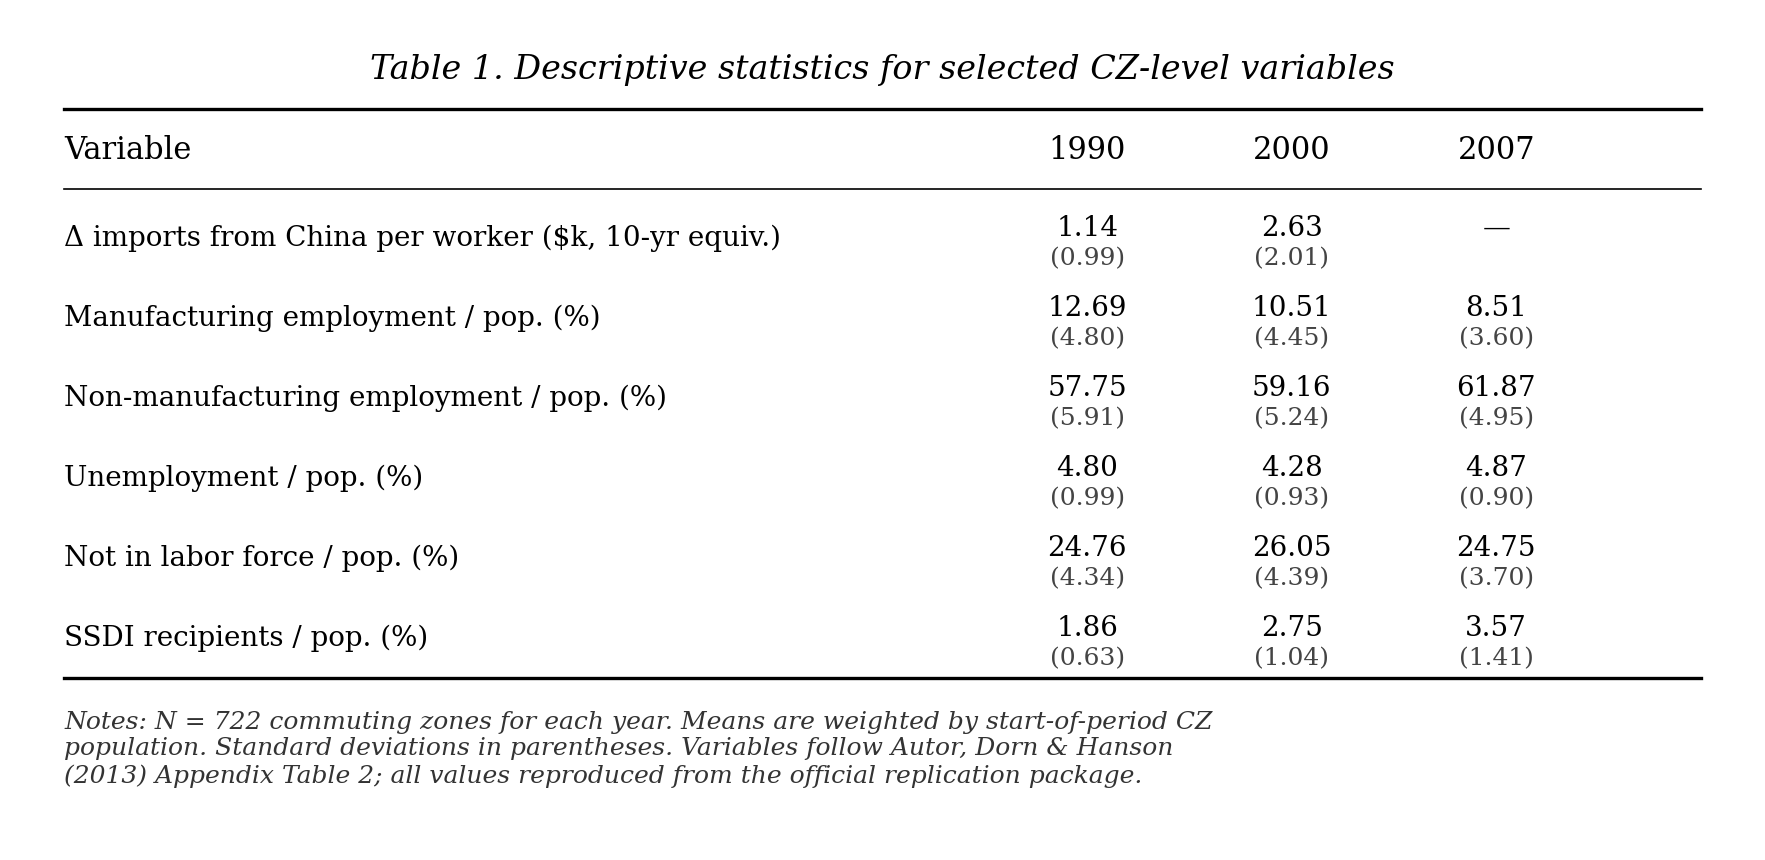
\includegraphics[width=1\linewidth,height=\textheight,keepaspectratio]{assets/yuxiao_table1.png}

}

\caption{\label{fig-yuxiao-summary}Descriptive statistics for selected
CZ-level variables, reproduced from ADH 2013 Appendix Table 2.}

\end{figure}%

\section{Analysis and Findings}\label{analysis-and-findings}

\subsection{Identification Strategy and its
Plausibility}\label{identification-strategy-and-its-plausibility}

OLS estimation of the labor-market effect of Chinese import exposure
faces an endogeneity problem. Observed U.S. imports reflect both Chinese
supply-side and U.S. demand shocks, biasing OLS toward zero. ADH (2013)
report an OLS estimate of −0.171 versus an IV estimate of −0.596
(\citeproc{ref-autorDornHanson2013}{Autor et al. 2013}).

They address this with a Bartik-style instrument, replacing
\(\Delta IPW_{uit}\) with \(\Delta IPW_{oit}\), built from same-period
Chinese exports to eight other high-income countries (Australia,
Denmark, Finland, Germany, Japan, New Zealand, Spain, and Switzerland).
The identifying assumption is that within-industry import growth shared
by these countries reflects China's supply-side improvements, not
correlated demand:

\[
\Delta IPW_{uit}=\sum_j \left(\frac{L_{ijt}}{L_{ujt}}\right)\cdot \left(\frac{\Delta M_{ucjt}}{L_{it}}\right),
\]

\[
\Delta IPW_{oit}=\sum_j \left(\frac{L_{ij,t-1}}{L_{uj,t-1}}\right)\cdot \left(\frac{\Delta M_{ocjt}}{L_{i,t-1}}\right).
\]

The second-stage equation is estimated as stacked first differences:

\[
\Delta L_{itm}=\gamma_t+\beta_1\Delta IPW_{uit}+X_{it}'\beta_2+e_{it},
\]

where \(X_{it}\) contains start-of-period manufacturing share,
demographic controls, the routine and offshorability indices of Autor
and Dorn (2013), and Census division dummies
(\citeproc{ref-autorDorn2013}{Autor and Dorn 2013}).

Three pieces of evidence support the strategy. First, the first stage is
strong: the instrument predicts the endogenous regressor with
coefficient 0.631 (\(t=6.90\)), well above the weak-IV threshold.
Second, a falsification test shows that 1970s--1980s manufacturing
changes do not predict future Chinese exposure, ruling out a
pre-existing decline. Third, dropping suspect industries leaves the
coefficient near −0.596.

The main residual concern is correlated demand shocks across high-income
economies. A gravity-based check yields similar estimates; Chinese
manufacturing TFP grew about 8\% per year over 1998--2007, against 3.9\%
in the U.S., supporting the supply-driven interpretation.

\subsection{Reproduction of Published
Results}\label{reproduction-of-published-results}

We verify that the official replication package functions correctly. Our
target is Table 3 of ADH (2013), the 2SLS regression of CZ-level change
in manufacturing employment share on \(\Delta IPW_{uit}\), instrumented
by the eight-country measure. We focus on column (6) with full controls.

Running the official Stata code on the published workfile, we obtain
coefficients matching the published values exactly to three decimal
places across all six columns. In column (6), the coefficient on
\(\Delta IPW\) is −0.596 (SE 0.099); the first-stage coefficient is
0.631 (\(t=6.90\)); \(N=1{,}444\) with \(R^2=0.343\). Table
Figure~\ref{fig-yuxiao-replication} reports the full comparison.

\begin{figure}[H]

\centering{

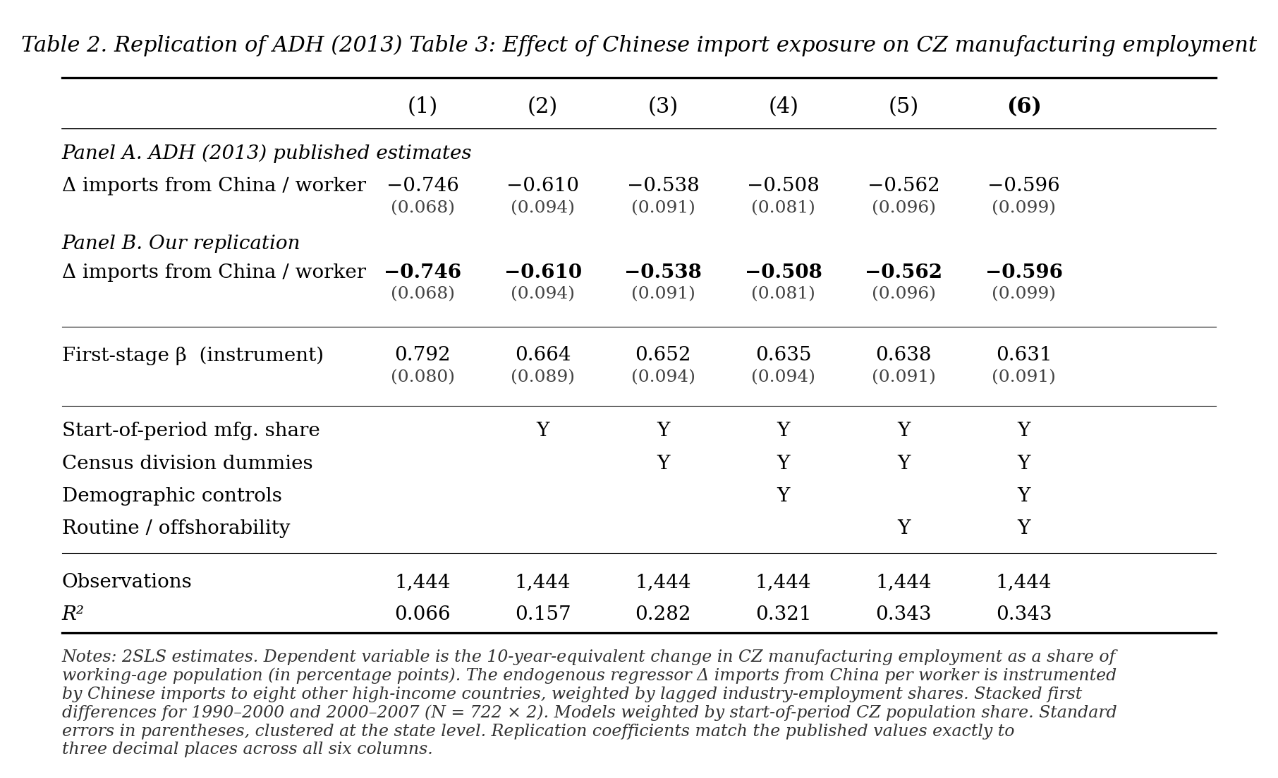
\includegraphics[width=1\linewidth,height=\textheight,keepaspectratio]{assets/yuxiao_table2.png}

}

\caption{\label{fig-yuxiao-replication}Replication of ADH (2013) Table 3
--- effect of Chinese import exposure on CZ manufacturing employment
share.}

\end{figure}%

Economically, −0.596 implies that a \$1,000 per-worker increase in
decadal Chinese exposure lowers a CZ's manufacturing share by 0.6
percentage points. ADH attribute 44\% of the 1990--2007 manufacturing
decline to this channel. Because we use the original data and code, this
is a computational reproduction---the exact match confirms our codebase
functions correctly. The next section applies the same strategy to
CZ-level presidential political outcomes.

\subsection{Extension: Dynamic Political Effects of the China
Shock}\label{extension-dynamic-political-effects-of-the-china-shock}

We extend the ADH local-labor-market design to presidential political
outcomes. The outcome is the Republican presidential vote margin in CZ
\(c\) and election year \(t\). The preferred specification includes CZ
fixed effects, election-year fixed effects, the ADH 1990--2007
import-exposure measure interacted with election-year indicators, and
time-varying effects of baseline controls. The omitted year is 1988, so
coefficients describe how the relationship between China-shock exposure
and Republican margin changes relative to the pre-shock election
immediately before the main exposure period.

A central measurement challenge is that electoral data are observed for
counties whose boundaries change over time, while ADH exposure is
measured for 1990 commuting zones. We therefore bridge county election
returns to 1990 counties using the FTZ county crosswalks, aggregate
counties to 1990 CZs using the Tolbert-Sizer/USDA crosswalk, and merge
those outcomes to ADH exposure. Our preferred bridge uses FTZ M5 weights
where available and M2 fallback weights where M5 is undefined or zero.
We validate retained vote shares, document fallback counties, and
compare the results to M6+fallback, pure M2, and M4+fallback. These
checks are important because the estimates should not be driven by
arbitrary geographic harmonization choices.

The empirical exercise should be interpreted as a reduced-form exposure
design, not as definitive evidence of individual belief updating. ADH
exposure is a shift-share measure: CZs differ in initial industry
composition, and industries differ in later import growth.
Identification requires either that initial industry shares are
conditionally unrelated to counterfactual political trends, or that the
industry-level import shifts are as-good-as-random with respect to local
political trends
(\citeproc{ref-goldsmithPinkhamSorkinSwift2020}{Goldsmith-Pinkham et al.
2020}; \citeproc{ref-borusyakHullJaravel2025}{Borusyak et al. 2025}).
These assumptions are not innocuous. In our diagnostics, the ADH
instrument strongly predicts exposure, but exposure is also highly
correlated with baseline manufacturing intensity and routine-task
concentration. Table Table~\ref{tbl-bartik-firststage} summarizes the
first-stage strength in our political-outcome sample.

{

\begin{longtable}[]{@{}lrrrr@{}}

\caption{\label{tbl-bartik-firststage}First-stage diagnostics for ADH
exposure.}

\tabularnewline

\toprule\noalign{}
Specification & Estimate & Std. error & First-stage F & N \\
\midrule\noalign{}
\endhead
\bottomrule\noalign{}
\endlastfoot
Minimal & 0.977 & 0.085 & 133.4 & 722 \\
Core controls & 0.812 & 0.101 & 64.6 & 722 \\
Full controls & 0.794 & 0.101 & 62.0 & 722 \\

\end{longtable}

}

Figure Figure~\ref{fig-main-event-study} presents the main event-study
estimates. The preferred inference is CZ-clustered. Conley,
Driscoll-Kraay, Newey-West, state-clustered, and two-way clustered
alternatives are computed as diagnostics, but several spatial and
two-way variance-covariance matrices are non-positive-definite or
require numerical repair in this short election-year panel. We therefore
state the conclusions cautiously and base the main figure on
CZ-clustered confidence intervals.

\begin{figure}[H]

\centering{

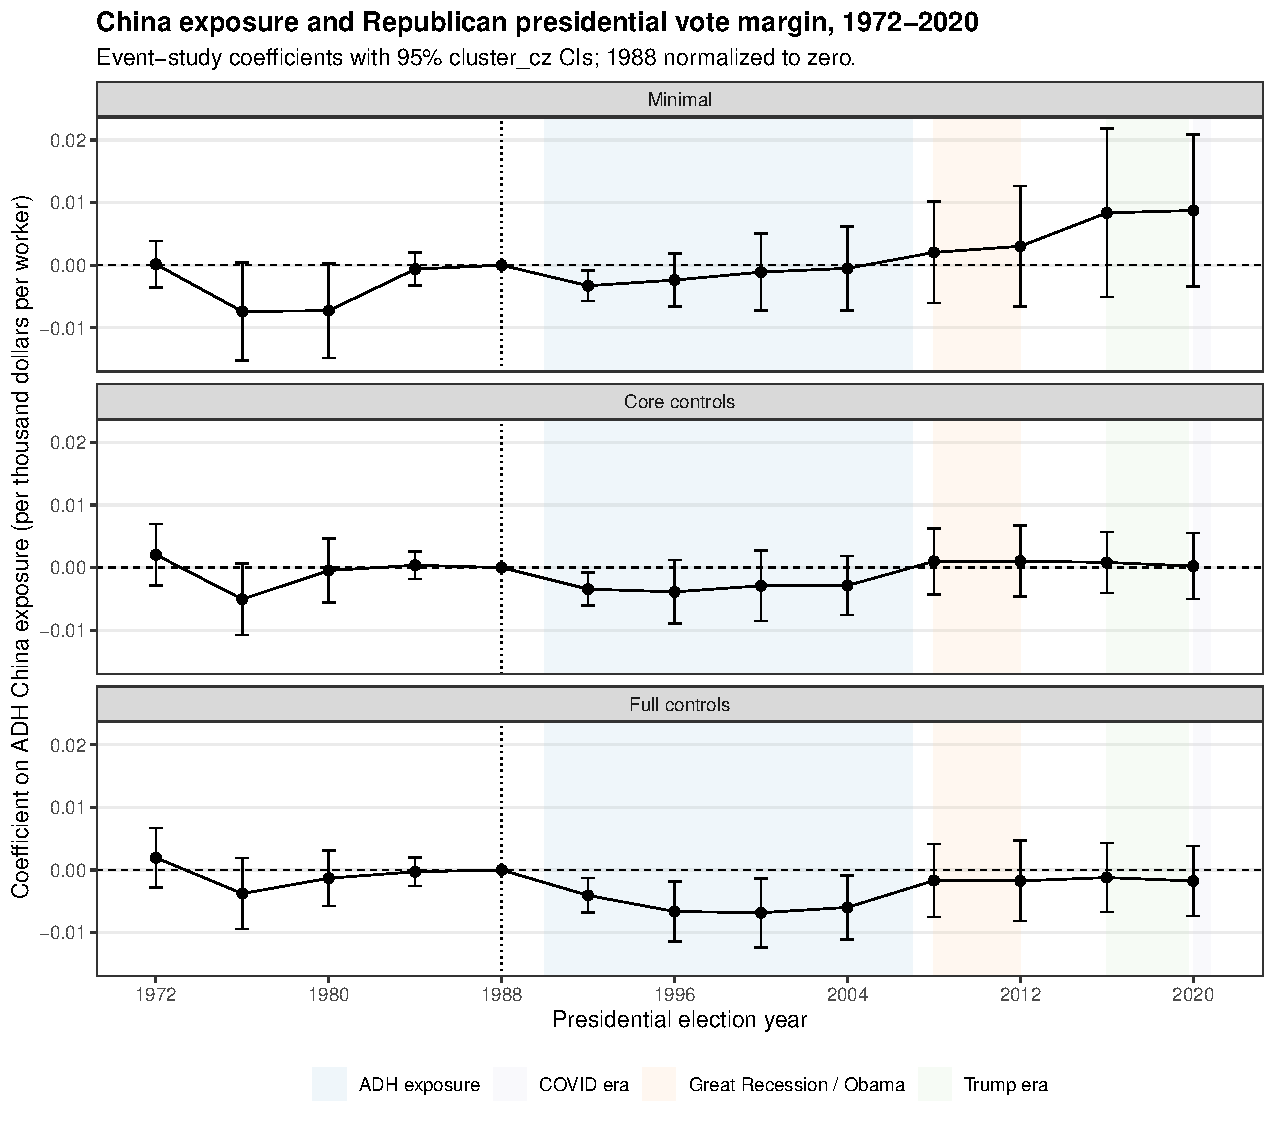
\includegraphics[width=1\linewidth,height=\textheight,keepaspectratio]{../output/figures/fig_event_study_rep_margin_main_specs_m5.pdf}

}

\caption{\label{fig-main-event-study}Event-study coefficients for ADH
exposure and Republican presidential margin.}

\end{figure}%

The estimates suggest little clear evidence of rising Republican margins
before the shock. The post-shock pattern is more consistent with a later
political response: the positive association grows in the medium and
long run, especially around the 2016 and 2020 horizons. This timing is
important because it suggests that the political effects of local trade
exposure may not operate immediately through local material losses
alone. They may also depend on later national political rhetoric, elite
positioning, media narratives, or changing turnout and party coalitions.

To understand what is behind the margin effect, we decompose the outcome
into Republican votes per 1990 population, Democratic votes per 1990
population, and two-party vote volume. Figure
Figure~\ref{fig-alt-decomp} shows that the margin pattern should not be
interpreted mechanically as a simple increase in Republican votes. The
broader decomposition helps distinguish vote-choice changes from changes
in participation and party-specific mobilization.

\begin{figure}[H]

\centering{

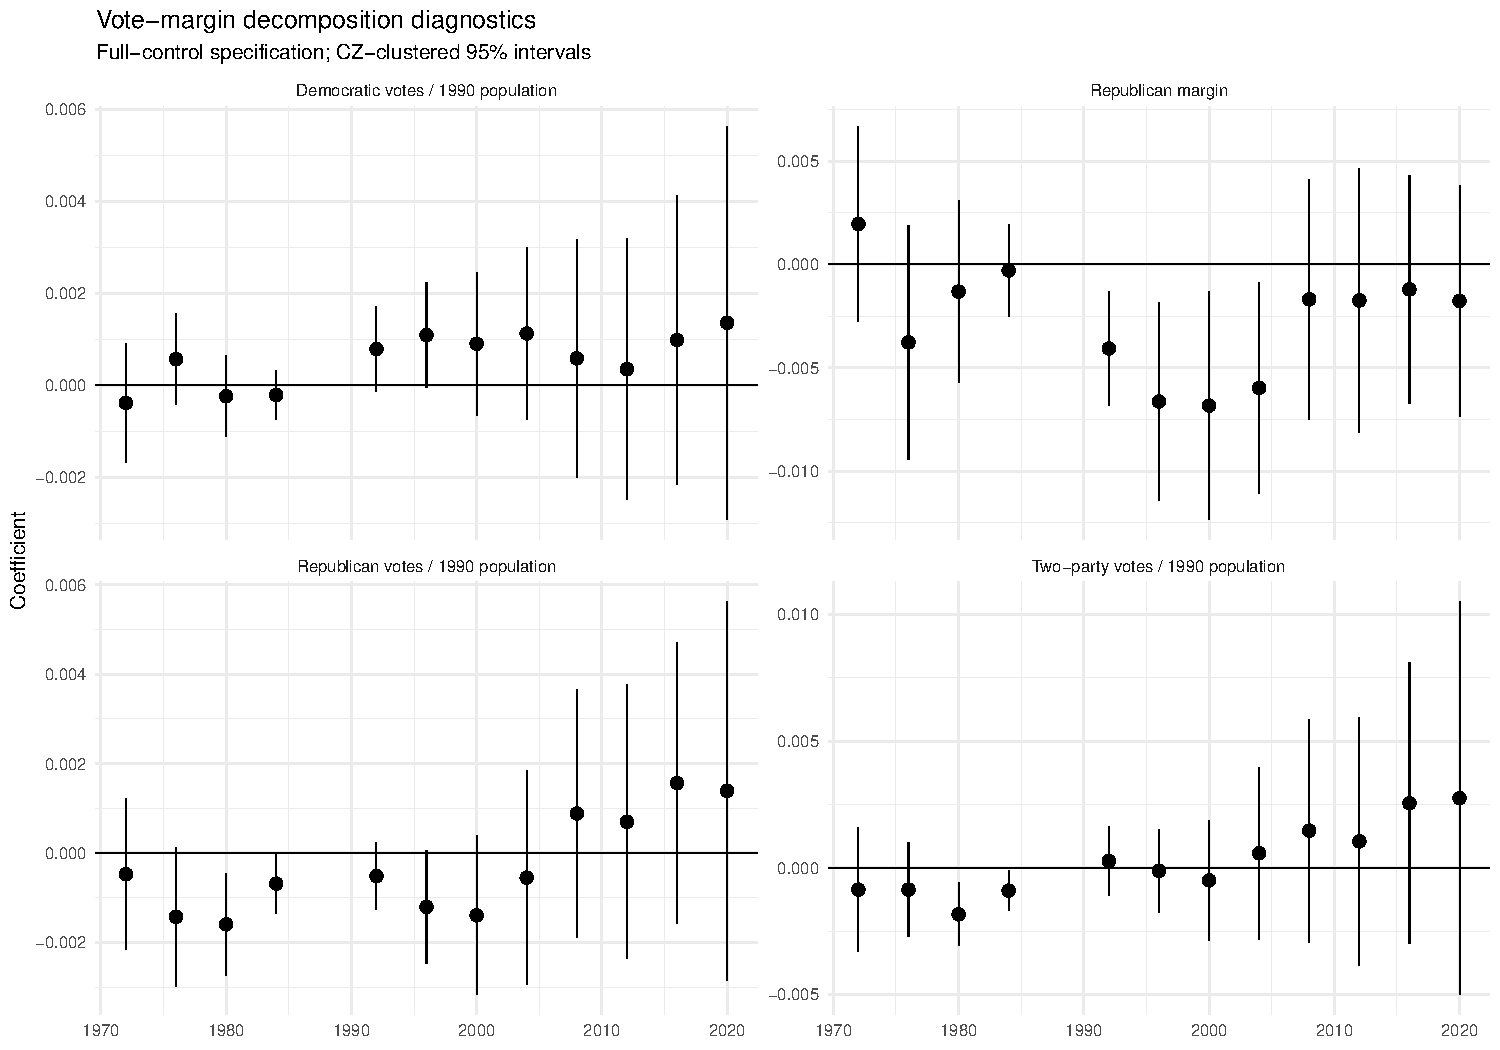
\includegraphics[width=1\linewidth,height=\textheight,keepaspectratio]{../output/figures/fig_alternative_political_outcome_decomposition.pdf}

}

\caption{\label{fig-alt-decomp}Political-outcome decomposition across
election years.}

\end{figure}%

Finally, we examine whether the single 1990--2007 exposure measure masks
important timing differences. The original ADH exposure measure
aggregates the China shock over a long period, so an event-study
coefficient for 2016 does not mean that a new trade shock occurs in
2016. It means that CZs with greater cumulative exposure by 2007 evolved
differently by 2016. To make this interpretation more transparent, we
split exposure into 1990--2000 and 2000--2007 components and include
both components jointly. Figure Figure~\ref{fig-subperiod-exposure}
shows that the estimated relationship varies depending on which
subperiod of import growth is emphasized. Pre-1988 coefficients in this
exercise are placebo relationships with future exposure, while post-2008
coefficients describe how early- and late-shock exposure predict later
political differences.

\begin{figure}[H]

\centering{

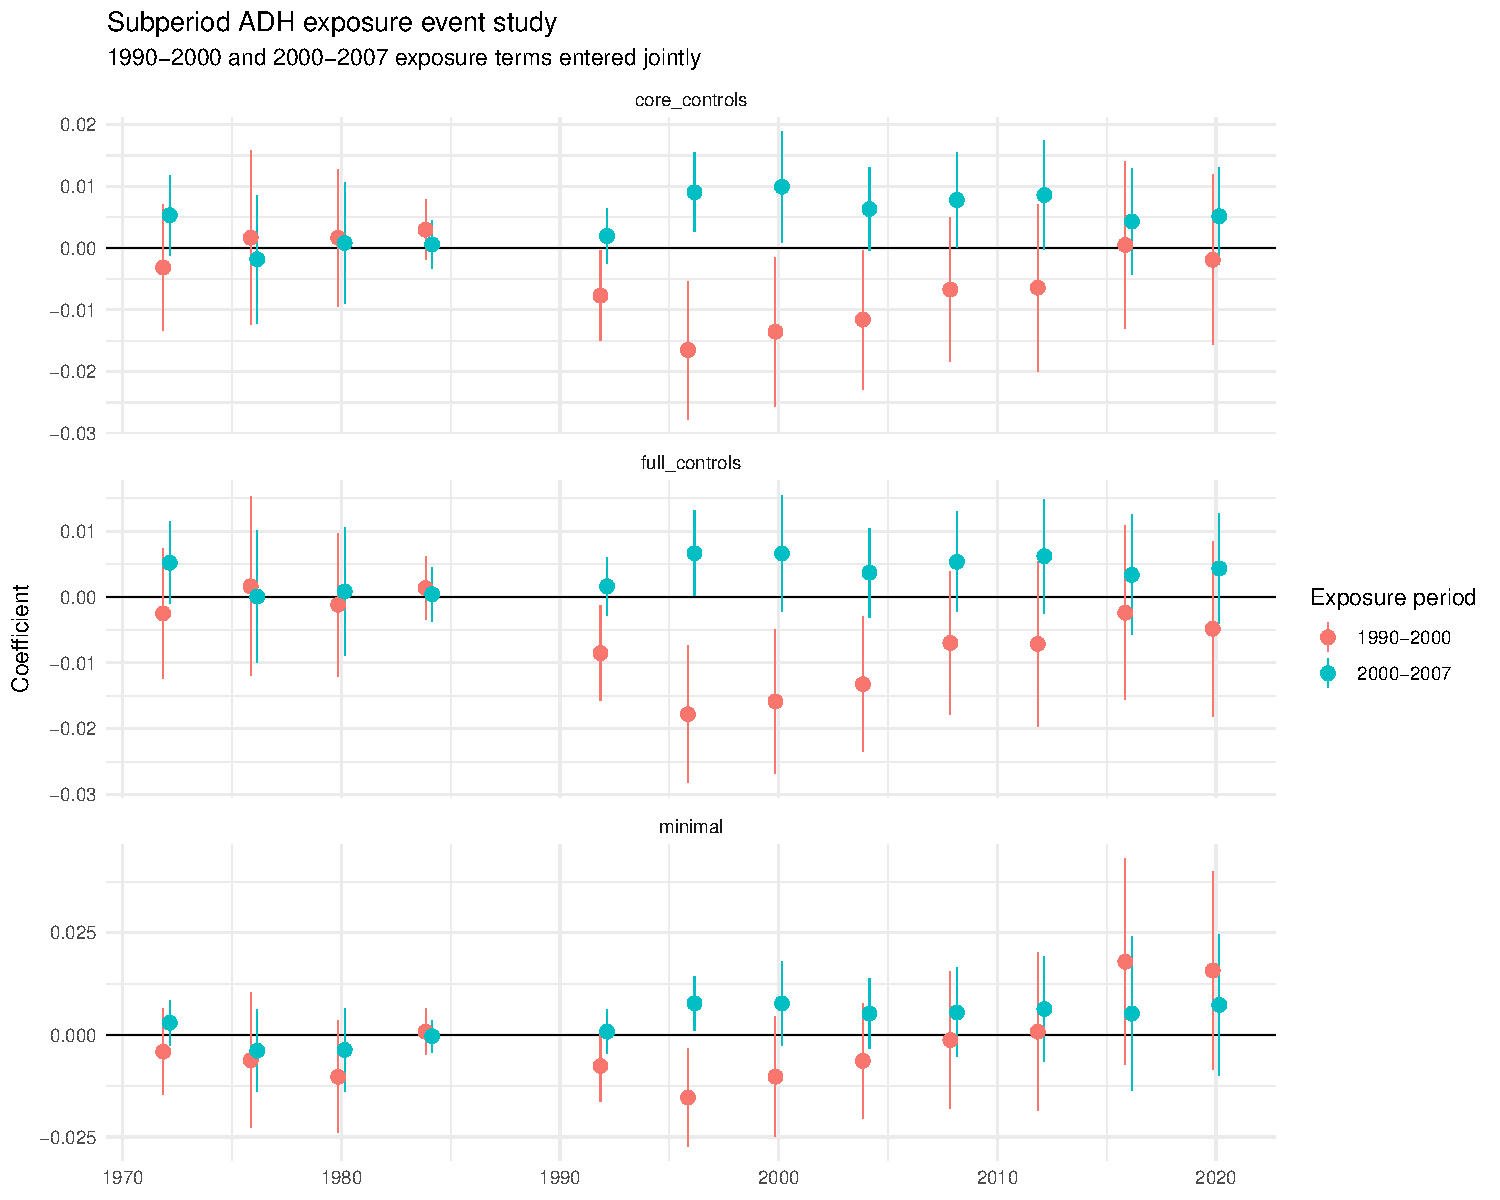
\includegraphics[width=1\linewidth,height=\textheight,keepaspectratio]{../output/figures/fig_subperiod_exposure_event_study.pdf}

}

\caption{\label{fig-subperiod-exposure}Subperiod ADH exposure event
study, with 1990--2000 and 2000--2007 exposure terms entered jointly.}

\end{figure}%

\section{Conclusion}\label{conclusion}

Our results suggest that the China shock may have had political
consequences beyond its direct effects on manufacturing employment. CZs
more exposed to Chinese import competition eventually show more
Republican-leaning presidential outcomes, with the clearest differences
appearing after the original labor-market shock rather than immediately.
This timing makes the interpretation complex. The estimates may reflect
voters responding to material local losses, but they may also reflect
later elite rhetoric, media framing, turnout changes, candidate supply,
or changes in local population composition.

The main lesson is that trade policy cannot be evaluated only through
employment and wage effects. Large local labor-market shocks may also
affect political representation, polarization, and support for future
policy regimes. At the same time, our conclusions should be cautious.
The design builds on a Bartik-style exposure measure, so interpretation
depends on assumptions about initial industry composition and
industry-level shocks. The unit of analysis is a commuting zone, not an
individual voter, so we cannot directly observe individual belief
updating. Our evidence is most informative about how local political
outcomes evolve in places more exposed to import competition, not about
a single definitive psychological mechanism.

Future work should therefore focus on mechanism. Turnout and
registration data, partisan-index data, migration data, and measures of
elite political supply could help distinguish material-experience
channels from mobilization, composition, and rhetoric/media channels.
Even with these limitations, the evidence suggests that the political
effects of globalization are dynamic, geographically concentrated, and
potentially mediated by institutions and narratives long after the
initial economic shock.

\section{References}\label{references}

\protect\phantomsection\label{refs}
\begin{CSLReferences}{1}{1}
\bibitem[\citeproctext]{ref-amlaniAlgara2021}
Amlani, Sharif, and Carlos Algara. 2021. {``Partisanship and
Nationalization in American Elections: Evidence from Presidential,
Senatorial, and Gubernatorial Elections in the u.s. Counties,
1872--2020.''} \emph{Electoral Studies} 73: 102387.
\url{https://doi.org/10.1016/j.electstud.2021.102387}.

\bibitem[\citeproctext]{ref-autorDorn2013}
Autor, David H., and David Dorn. 2013. {``The Growth of Low-Skill
Service Jobs and the Polarization of the US Labor Market.''}
\emph{American Economic Review} 103 (5): 1553--97.
\url{https://doi.org/10.1257/aer.103.5.1553}.

\bibitem[\citeproctext]{ref-autorDornHanson2013}
Autor, David H., David Dorn, and Gordon H. Hanson. 2013. {``The China
Syndrome: Local Labor Market Effects of Import Competition in the United
States.''} \emph{American Economic Review} 103 (6): 2121--68.
\url{https://doi.org/10.1257/aer.103.6.2121}.

\bibitem[\citeproctext]{ref-borusyakHullJaravel2025}
Borusyak, Kirill, Peter Hull, and Xavier Jaravel. 2025. {``Design-Based
Identification with Formula Instruments: A Review.''} \emph{Journal of
Economic Perspectives} 39 (2): 157--80.
\url{https://doi.org/10.1257/jep.20231370}.

\bibitem[\citeproctext]{ref-ferraraTestaZhou2024}
Ferrara, Andreas, Patrick A. Testa, and Liyang Zhou. 2024. {``Crosswalks
for u.s. Counties and Congressional Districts, 1790--2020.''}
\emph{Historical Methods: A Journal of Quantitative and
Interdisciplinary History}, ahead of print.
\url{https://doi.org/10.1080/01615440.2024.2369230}.

\bibitem[\citeproctext]{ref-goldsmithPinkhamSorkinSwift2020}
Goldsmith-Pinkham, Paul, Isaac Sorkin, and Henry Swift. 2020. {``Bartik
Instruments: What, When, Why, and How.''} \emph{American Economic
Review} 110 (8): 2586--624. \url{https://doi.org/10.1257/aer.20181047}.

\bibitem[\citeproctext]{ref-tolbertSizer1996}
Tolbert, Charles M., and Molly Sizer. 1996. \emph{U.s. Commuting Zones
and Labor Market Areas: A 1990 Update}. Economic Research Service, U.S.
Department of Agriculture.

\bibitem[\citeproctext]{ref-usdaERSCommutingZones}
U.S. Department of Agriculture Economic Research Service. 2026.
\emph{Commuting Zones and Labor Market Areas}. Data product.

\end{CSLReferences}

\newpage
\appendix

\section{Appendix A: County-to-CZ Harmonization and
Measurement}\label{appendix-a-county-to-cz-harmonization-and-measurement}

This appendix documents the county-to-CZ bridge used to construct
political outcomes. County election returns are bridged to 1990 counties
using FTZ crosswalk weights and then aggregated to 1990 CZs. The
preferred design uses M5 where valid and M2 fallback where M5 is
undefined or zero.

{

\begin{longtable}[]{@{}
  >{\raggedright\arraybackslash}p{(\linewidth - 10\tabcolsep) * \real{0.1833}}
  >{\raggedright\arraybackslash}p{(\linewidth - 10\tabcolsep) * \real{0.0300}}
  >{\raggedright\arraybackslash}p{(\linewidth - 10\tabcolsep) * \real{0.0200}}
  >{\raggedleft\arraybackslash}p{(\linewidth - 10\tabcolsep) * \real{0.0300}}
  >{\raggedleft\arraybackslash}p{(\linewidth - 10\tabcolsep) * \real{0.0367}}
  >{\raggedright\arraybackslash}p{(\linewidth - 10\tabcolsep) * \real{0.7000}}@{}}

\caption{\label{tbl-validation-checks}Pipeline validation checks.}

\tabularnewline

\toprule\noalign{}
\begin{minipage}[b]{\linewidth}\raggedright
check
\end{minipage} & \begin{minipage}[b]{\linewidth}\raggedright
status
\end{minipage} & \begin{minipage}[b]{\linewidth}\raggedright
fatal
\end{minipage} & \begin{minipage}[b]{\linewidth}\raggedleft
n\_failed
\end{minipage} & \begin{minipage}[b]{\linewidth}\raggedleft
n\_reported
\end{minipage} & \begin{minipage}[b]{\linewidth}\raggedright
details
\end{minipage} \\
\midrule\noalign{}
\endhead
\bottomrule\noalign{}
\endlastfoot
adh\_one\_row\_per\_czone & pass & TRUE & 0 & NA & Requires one ADH
baseline/exposure row per commuting zone. \\
cz\_lookup\_unique\_1990\_counties & pass & TRUE & 0 & NA & Requires
each 1990 county FIPS to appear once and map to one CZ. \\
aa\_all\_county\_fips\_valid & pass & TRUE & 0 & NA & Requires all
county FIPS to be five numeric digits before filtering. \\
aa\_vote\_identity\_error\_within\_tolerance & pass & TRUE & 0 & NA &
Max absolute vote identity error: 0 \\
crosswalk\_positive\_final\_weight\_sums\_equal\_one & pass & TRUE & 0 &
NA & Tolerance: 1e-06 \\
crosswalk\_all\_source\_weight\_sums\_equal\_one\_or\_reported &
reported & FALSE & 0 & 162 & Global non-ADH or unsupported source-county
rows are reported rather than treated as validation failures. Estimation
is gated by positive final weights, retained vote share, and panel
balance. Tolerance: 1e-06 \\
crosswalk\_undefined\_selected\_weights\_handled & pass & TRUE & 1204 &
NA & Policy: fallback\_m2 \\
aa\_no\_duplicate\_county\_years\_after\_exact\_distinct & pass & TRUE &
0 & NA & Exact duplicate rows removed: 0 \\
aa\_two\_party\_votes\_match\_party\_votes & pass & TRUE & 0 & NA &
Requires republican + democratic votes to equal two-party votes. \\
aa\_votes\_nonnegative & pass & TRUE & 0 & NA & Requires nonnegative
Republican, Democratic, two-party, and total votes. \\
bridged\_vote\_retention\_above\_threshold & pass & TRUE & 0 & NA &
Minimum retained share in main years: 0.996122 \\
main\_panel\_balanced & pass & TRUE & 0 & NA & Observed complete rows:
9386; expected rows: 9386; missing share: 0 \\
event\_study\_residualized\_design\_full\_rank & pass & TRUE & 0 & NA &
Requires no residualized RHS rank deficiency in 1952-start or 1972-start
specifications. \\
event\_study\_main\_vcov\_available\_without\_repair & pass & TRUE & 0 &
NA & Main SE type: cluster\_cz \\
event\_study\_conley\_repair\_diagnostics\_recorded & pass & FALSE & 31
& NA & Conley VCOVs requiring repair across all samples/specs/cutoffs:
31 \\

\end{longtable}

}

{

\begin{longtable}[]{@{}
  >{\raggedleft\arraybackslash}p{(\linewidth - 8\tabcolsep) * \real{0.0641}}
  >{\raggedleft\arraybackslash}p{(\linewidth - 8\tabcolsep) * \real{0.2051}}
  >{\raggedleft\arraybackslash}p{(\linewidth - 8\tabcolsep) * \real{0.2308}}
  >{\raggedleft\arraybackslash}p{(\linewidth - 8\tabcolsep) * \real{0.2436}}
  >{\raggedright\arraybackslash}p{(\linewidth - 8\tabcolsep) * \real{0.2564}}@{}}

\caption{\label{tbl-retained-votes}Retained vote shares by year and
source scope.}

\tabularnewline

\toprule\noalign{}
\begin{minipage}[b]{\linewidth}\raggedleft
Year
\end{minipage} & \begin{minipage}[b]{\linewidth}\raggedleft
Source counties
\end{minipage} & \begin{minipage}[b]{\linewidth}\raggedleft
Fallback counties
\end{minipage} & \begin{minipage}[b]{\linewidth}\raggedleft
Unmatched counties
\end{minipage} & \begin{minipage}[b]{\linewidth}\raggedright
Retained vote share
\end{minipage} \\
\midrule\noalign{}
\endhead
\bottomrule\noalign{}
\endlastfoot
1972 & 3106 & 258 & 0 & 1.0000 \\
1976 & 3109 & 258 & 0 & 1.0000 \\
1980 & 3108 & 221 & 0 & 1.0000 \\
1984 & 3110 & 221 & 0 & 1.0000 \\
1988 & 3110 & 221 & 0 & 1.0000 \\
1992 & 3110 & 0 & 0 & 1.0000 \\
1996 & 3109 & 0 & 0 & 1.0000 \\
2000 & 3109 & 196 & 0 & 1.0000 \\
2004 & 3109 & 196 & 0 & 1.0000 \\
2008 & 3109 & 196 & 0 & 1.0000 \\
2012 & 3109 & 183 & 0 & 1.0000 \\
2016 & 3108 & 183 & 0 & 1.0000 \\
2020 & 3108 & 184 & 0 & 1.0000 \\

\end{longtable}

}

\begin{figure}[H]

\centering{

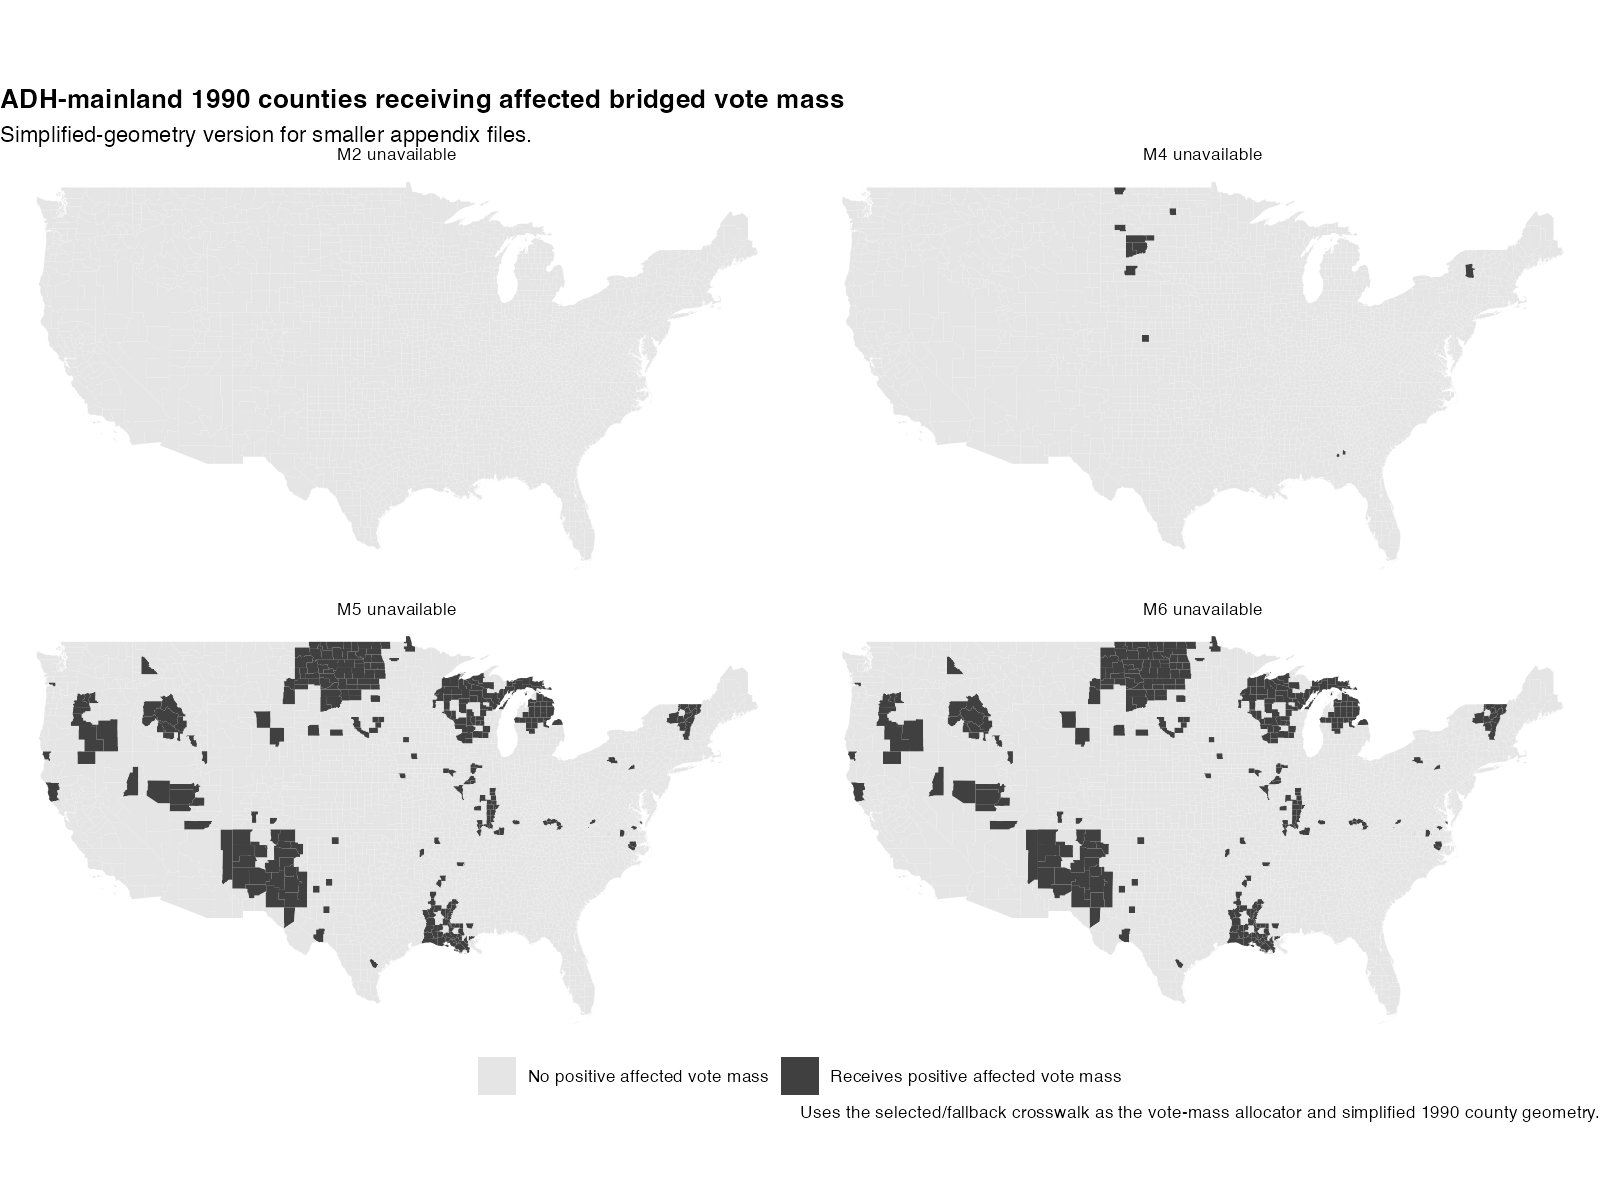
\includegraphics[width=1\linewidth,height=\textheight,keepaspectratio]{../output/figures/fig_crosswalk_unavailable_weights_1990_counties_small.png}

}

\caption{\label{fig-crosswalk-county-map}1990 counties receiving
positive vote mass from source counties with unavailable weights.}

\end{figure}%

\begin{figure}[H]

\centering{

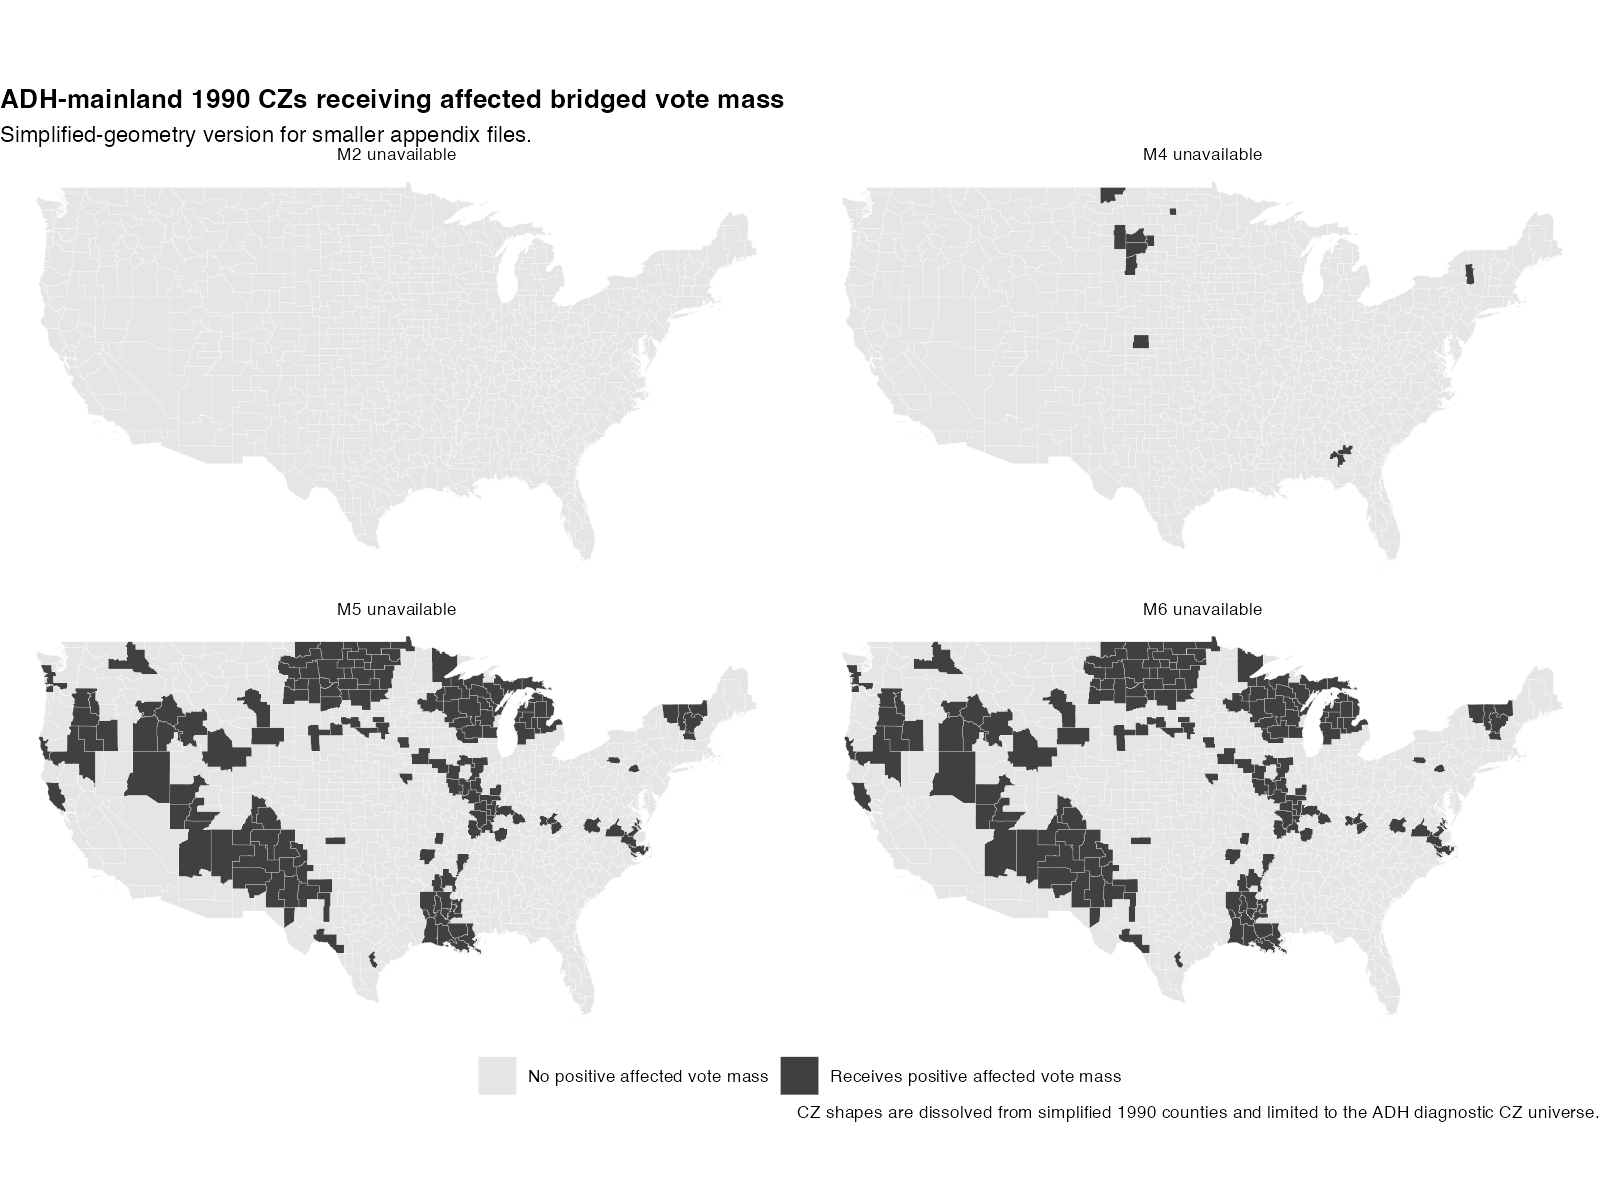
\includegraphics[width=1\linewidth,height=\textheight,keepaspectratio]{../output/figures/fig_crosswalk_unavailable_weights_1990_czs_small.png}

}

\caption{\label{fig-crosswalk-cz-map}1990 CZs receiving positive vote
mass from source counties with unavailable weights.}

\end{figure}%

\begin{figure}[H]

\centering{

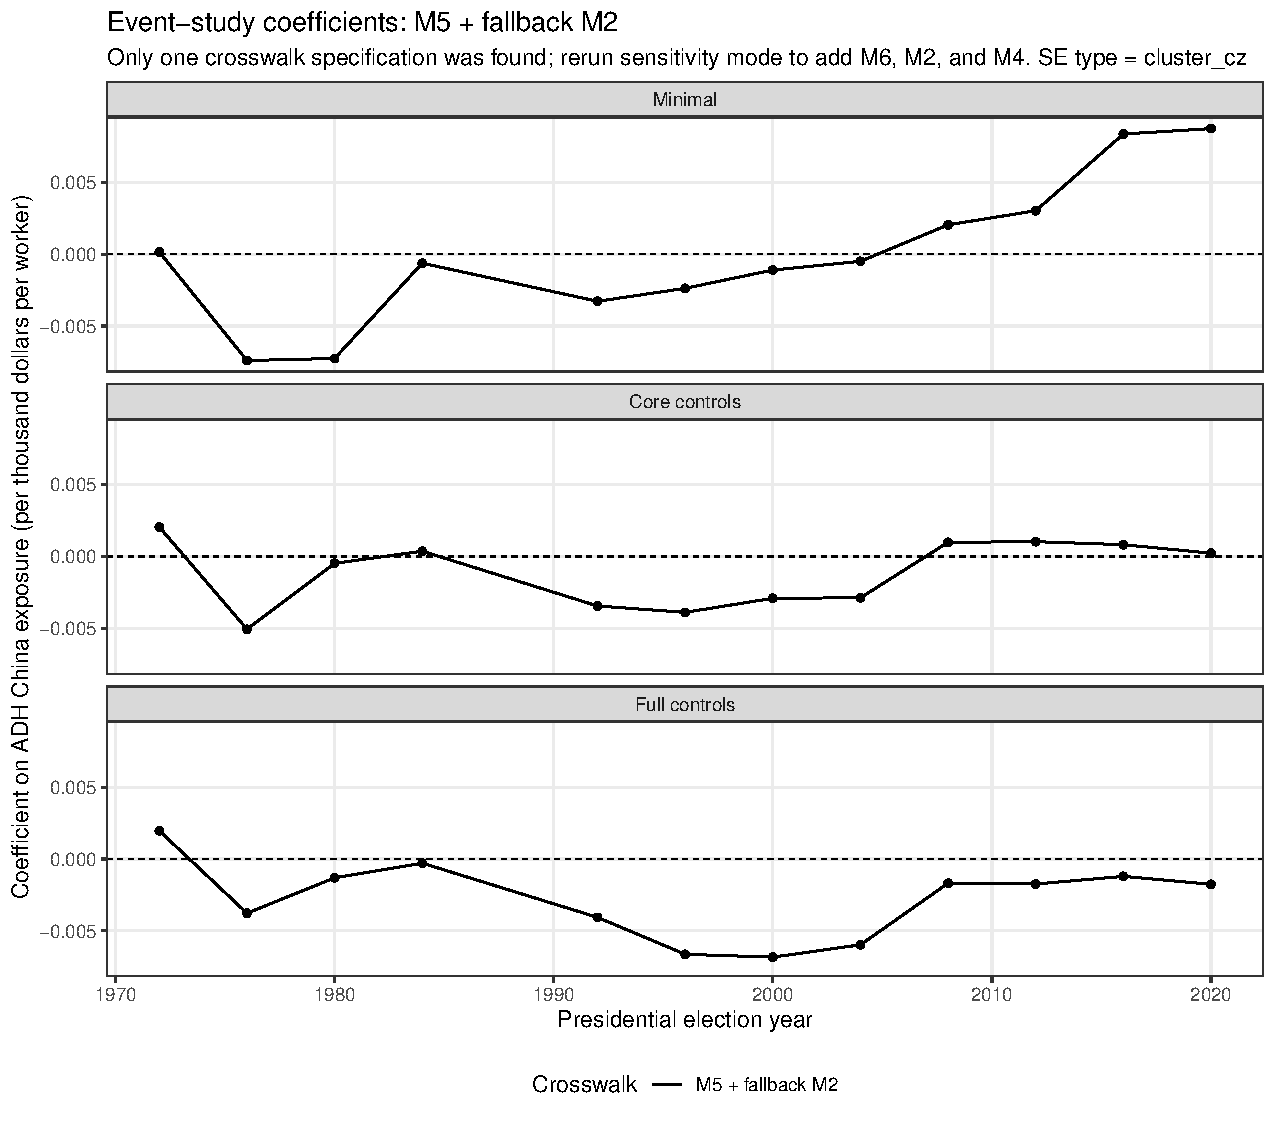
\includegraphics[width=1\linewidth,height=\textheight,keepaspectratio]{../output/figures/fig_crosswalk_specification_comparison.pdf}

}

\caption{\label{fig-crosswalk-comparison}Crosswalk-specification
comparison. If the full sensitivity pipeline has not been run, this
figure will show only the preferred M5+fallback design.}

\end{figure}%

\section{Appendix B: Main Event Study and Alternative Political
Outcomes}\label{appendix-b-main-event-study-and-alternative-political-outcomes}

{

\begin{longtable}[]{@{}
  >{\raggedright\arraybackslash}p{(\linewidth - 10\tabcolsep) * \real{0.2121}}
  >{\raggedleft\arraybackslash}p{(\linewidth - 10\tabcolsep) * \real{0.0758}}
  >{\raggedright\arraybackslash}p{(\linewidth - 10\tabcolsep) * \real{0.1364}}
  >{\raggedright\arraybackslash}p{(\linewidth - 10\tabcolsep) * \real{0.1667}}
  >{\raggedright\arraybackslash}p{(\linewidth - 10\tabcolsep) * \real{0.2879}}
  >{\raggedright\arraybackslash}p{(\linewidth - 10\tabcolsep) * \real{0.1212}}@{}}

\caption{\label{tbl-main-event-table}Main event-study coefficient table,
selected years.}

\tabularnewline

\toprule\noalign{}
\begin{minipage}[b]{\linewidth}\raggedright
Spec
\end{minipage} & \begin{minipage}[b]{\linewidth}\raggedleft
Year
\end{minipage} & \begin{minipage}[b]{\linewidth}\raggedright
Estimate
\end{minipage} & \begin{minipage}[b]{\linewidth}\raggedright
Std. error
\end{minipage} & \begin{minipage}[b]{\linewidth}\raggedright
95\% CI
\end{minipage} & \begin{minipage}[b]{\linewidth}\raggedright
p-value
\end{minipage} \\
\midrule\noalign{}
\endhead
\bottomrule\noalign{}
\endlastfoot
Minimal & 1972 & 0.0002 & 0.0019 & {[}-0.0036, 0.0039{]} & 0.936 \\
Minimal & 1992 & -0.0033 & 0.0012 & {[}-0.0057, -0.0008{]} & 0.009 \\
Minimal & 2000 & -0.0011 & 0.0031 & {[}-0.0073, 0.0051{]} & 0.726 \\
Minimal & 2008 & 0.0020 & 0.0041 & {[}-0.0061, 0.0101{]} & 0.621 \\
Minimal & 2016 & 0.0084 & 0.0069 & {[}-0.0051, 0.0218{]} & 0.224 \\
Minimal & 2020 & 0.0087 & 0.0062 & {[}-0.0034, 0.0209{]} & 0.159 \\
Core controls & 1972 & 0.0021 & 0.0025 & {[}-0.0029, 0.0070{]} &
0.412 \\
Core controls & 1992 & -0.0034 & 0.0013 & {[}-0.0061, -0.0008{]} &
0.011 \\
Core controls & 2000 & -0.0029 & 0.0029 & {[}-0.0085, 0.0027{]} &
0.313 \\
Core controls & 2008 & 0.0010 & 0.0027 & {[}-0.0043, 0.0063{]} &
0.713 \\
Core controls & 2016 & 0.0008 & 0.0025 & {[}-0.0041, 0.0057{]} &
0.740 \\
Core controls & 2020 & 0.0002 & 0.0027 & {[}-0.0050, 0.0055{]} &
0.930 \\
Full controls & 1972 & 0.0020 & 0.0024 & {[}-0.0028, 0.0067{]} &
0.419 \\
Full controls & 1992 & -0.0041 & 0.0014 & {[}-0.0068, -0.0013{]} &
0.004 \\
Full controls & 2000 & -0.0068 & 0.0028 & {[}-0.0123, -0.0013{]} &
0.015 \\
Full controls & 2008 & -0.0017 & 0.0030 & {[}-0.0075, 0.0041{]} &
0.569 \\
Full controls & 2016 & -0.0012 & 0.0028 & {[}-0.0068, 0.0043{]} &
0.668 \\
Full controls & 2020 & -0.0018 & 0.0029 & {[}-0.0074, 0.0038{]} &
0.537 \\

\end{longtable}

}

\begin{figure}[H]

\centering{

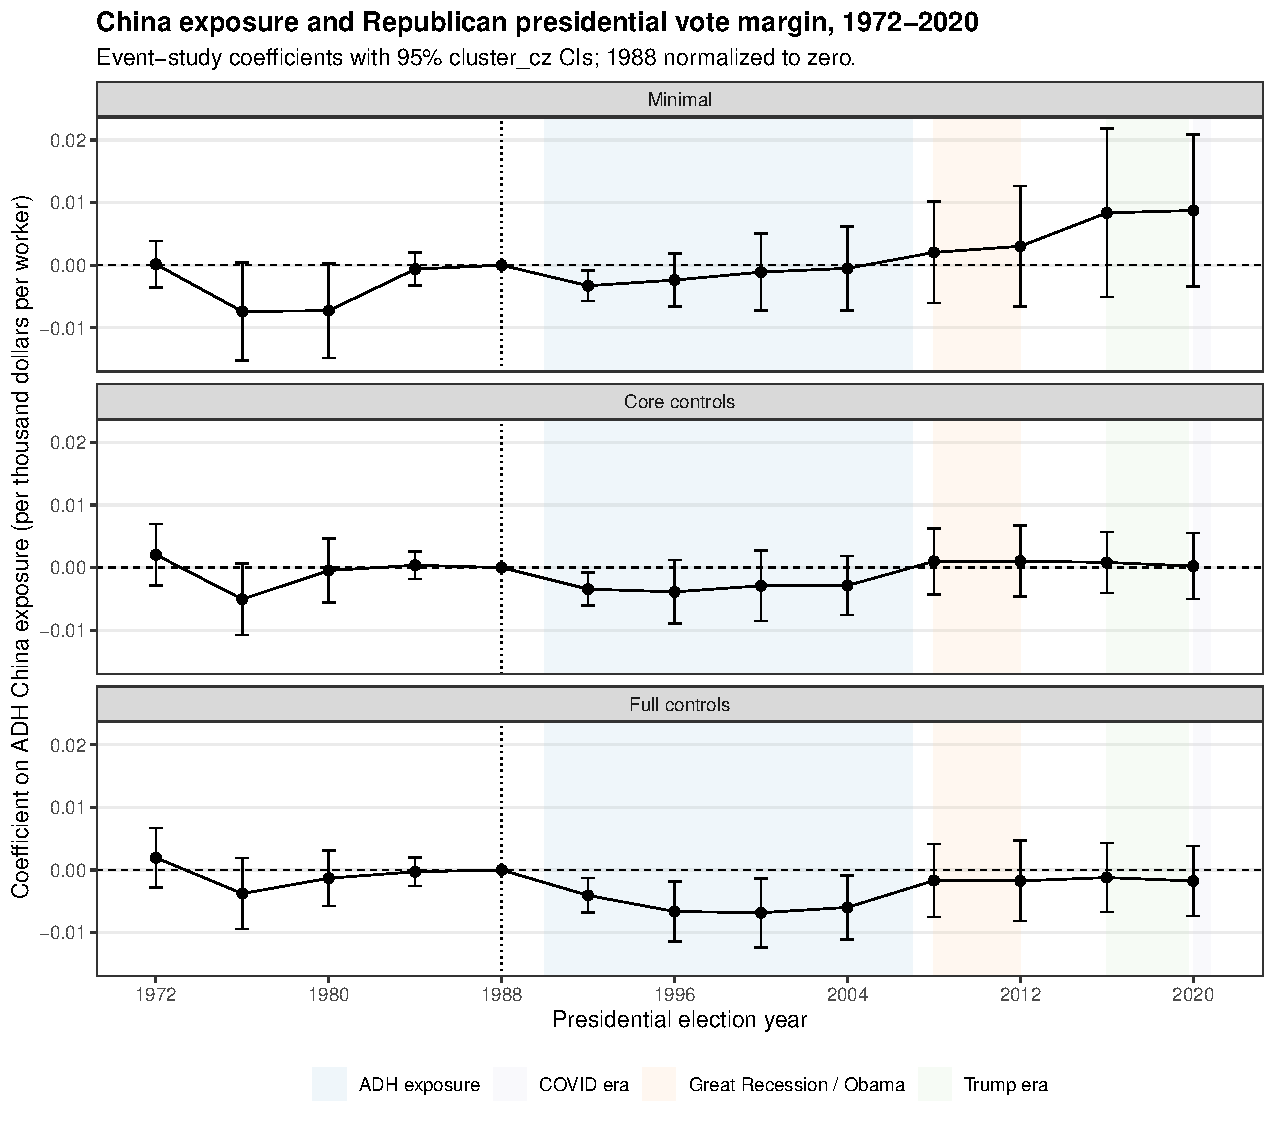
\includegraphics[width=1\linewidth,height=\textheight,keepaspectratio]{../output/figures/fig_event_study_rep_margin_main_specs_m5.pdf}

}

\caption{\label{fig-main-event-appendix}Main event-study estimates.}

\end{figure}%

\begin{figure}[H]

\centering{

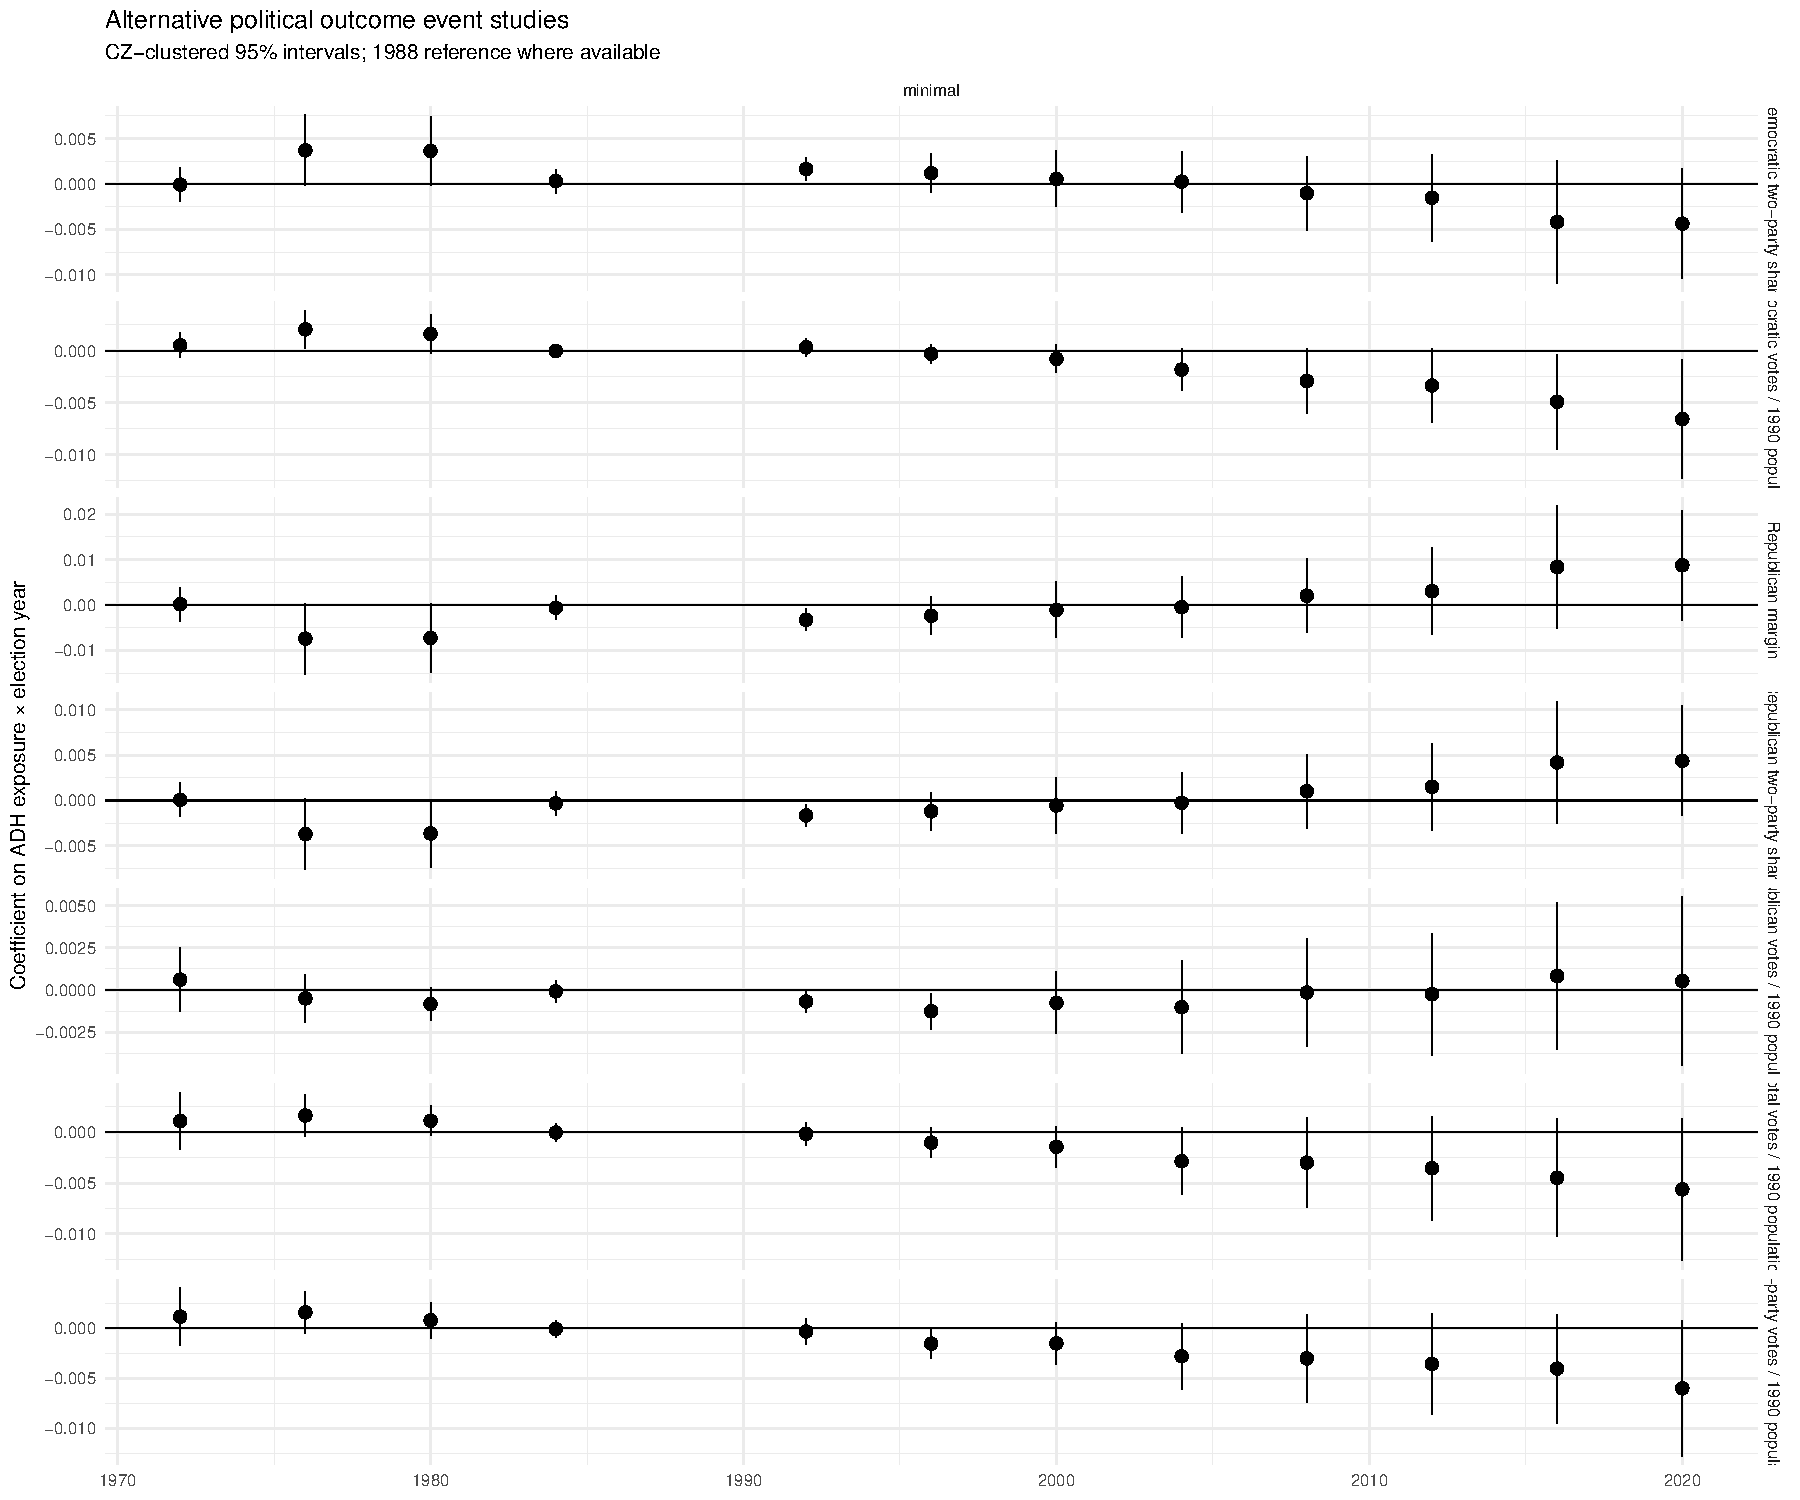
\includegraphics[width=1\linewidth,height=\textheight,keepaspectratio]{../output/figures/fig_alternative_political_outcomes.pdf}

}

\caption{\label{fig-alt-outcomes-full}Full alternative-outcome
event-study grid.}

\end{figure}%

\begin{figure}[H]

\centering{

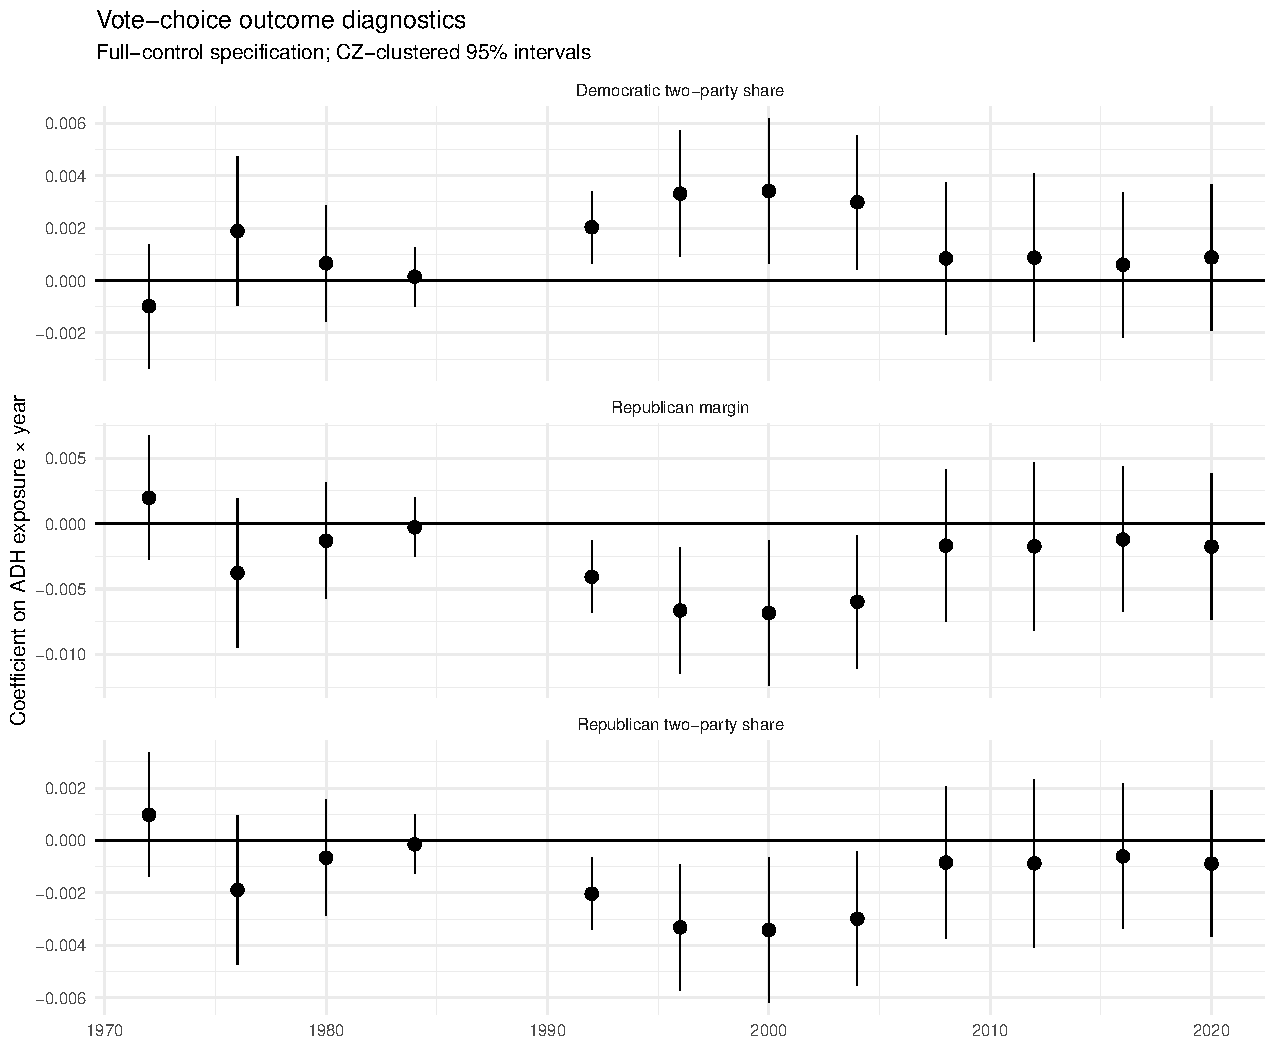
\includegraphics[width=1\linewidth,height=\textheight,keepaspectratio]{../output/figures/fig_alternative_political_outcomes_vote_choice.pdf}

}

\caption{\label{fig-alt-vote-choice}Vote-choice outcome family.}

\end{figure}%

\begin{figure}[H]

\centering{

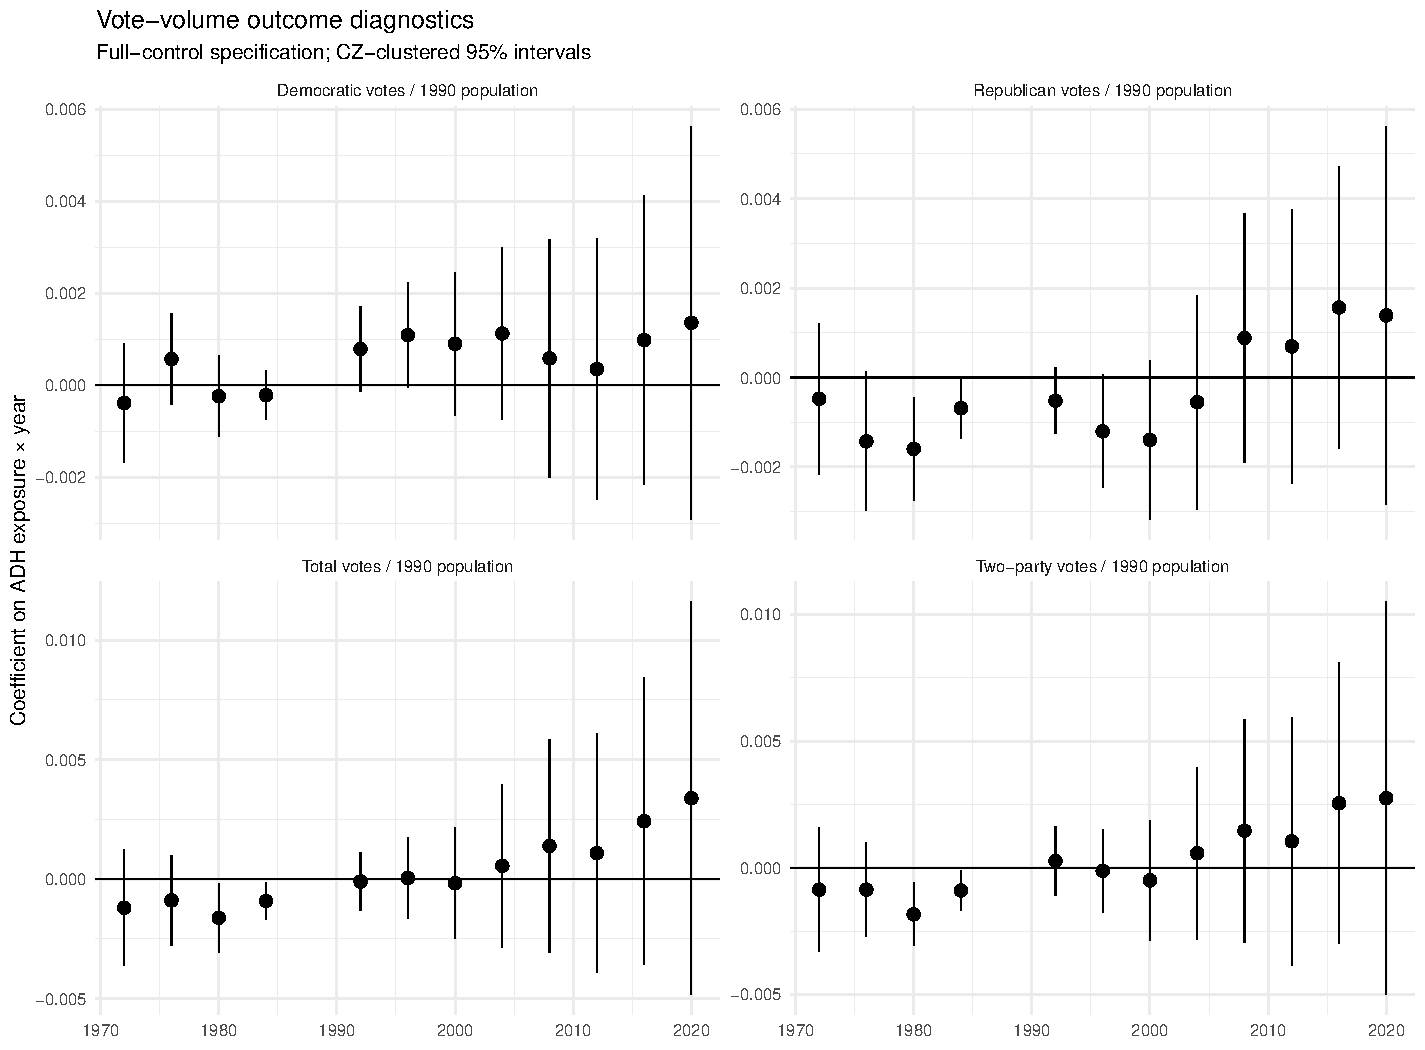
\includegraphics[width=1\linewidth,height=\textheight,keepaspectratio]{../output/figures/fig_alternative_political_outcomes_vote_volume.pdf}

}

\caption{\label{fig-alt-vote-volume}Vote-volume outcome family.}

\end{figure}%

\begin{figure}[H]

\centering{

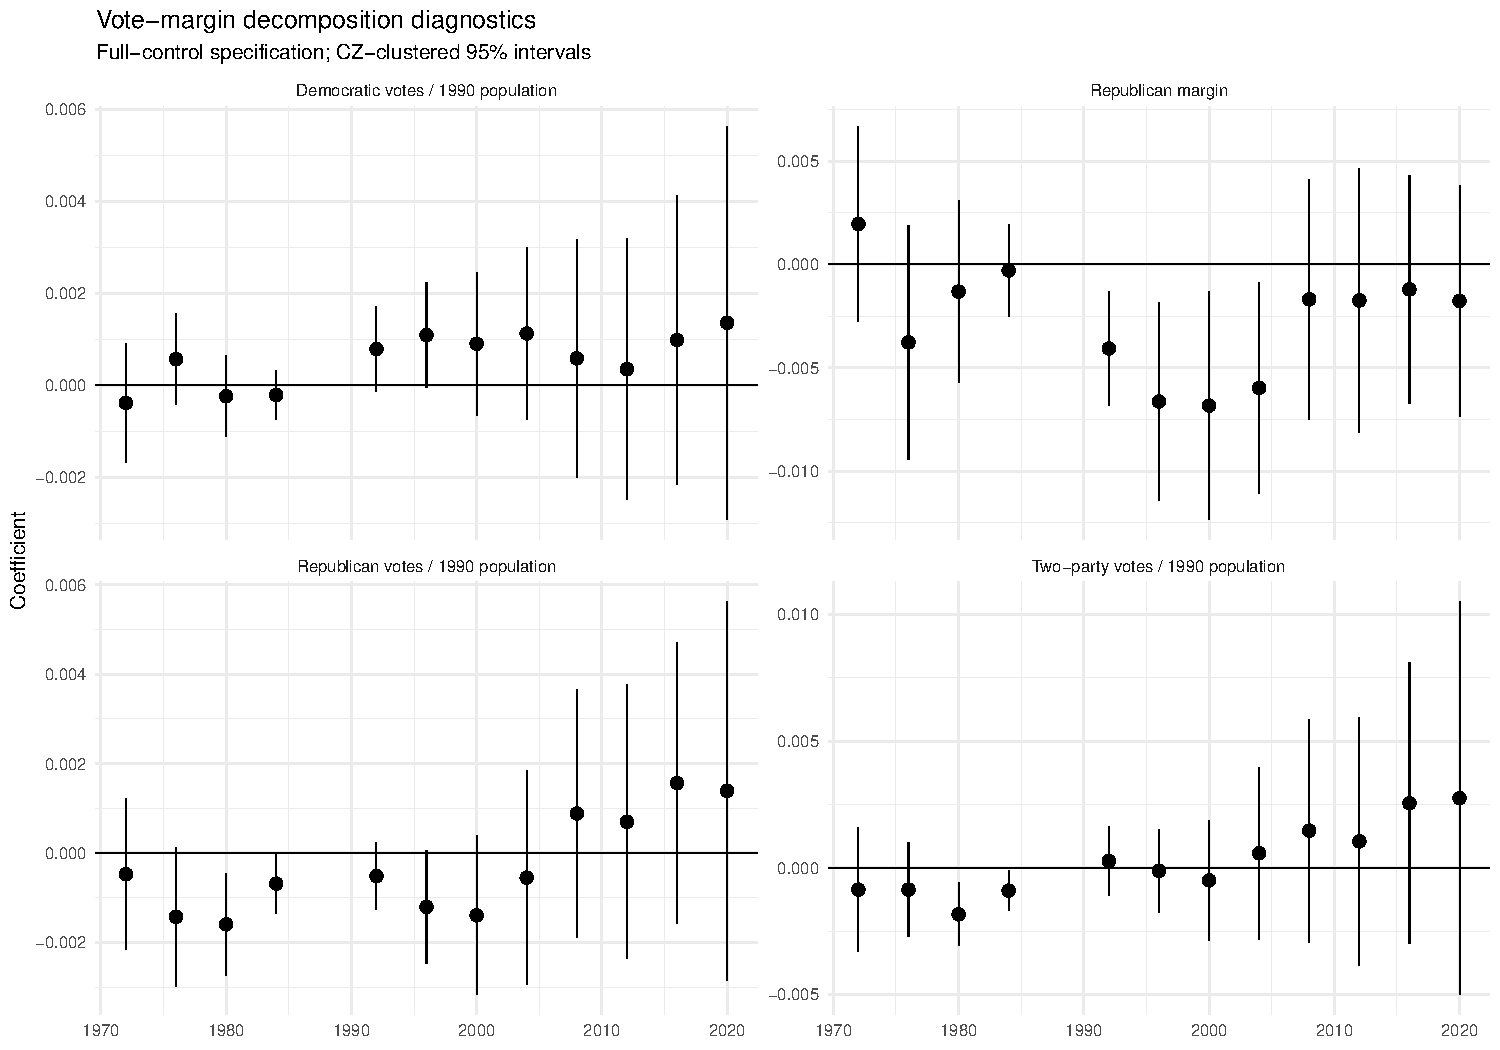
\includegraphics[width=1\linewidth,height=\textheight,keepaspectratio]{../output/figures/fig_alternative_political_outcome_decomposition.pdf}

}

\caption{\label{fig-alt-decomp-appendix}Outcome decomposition.}

\end{figure}%

\section{Appendix C: Bartik Identification
Diagnostics}\label{appendix-c-bartik-identification-diagnostics}

\begin{figure}[H]

\centering{

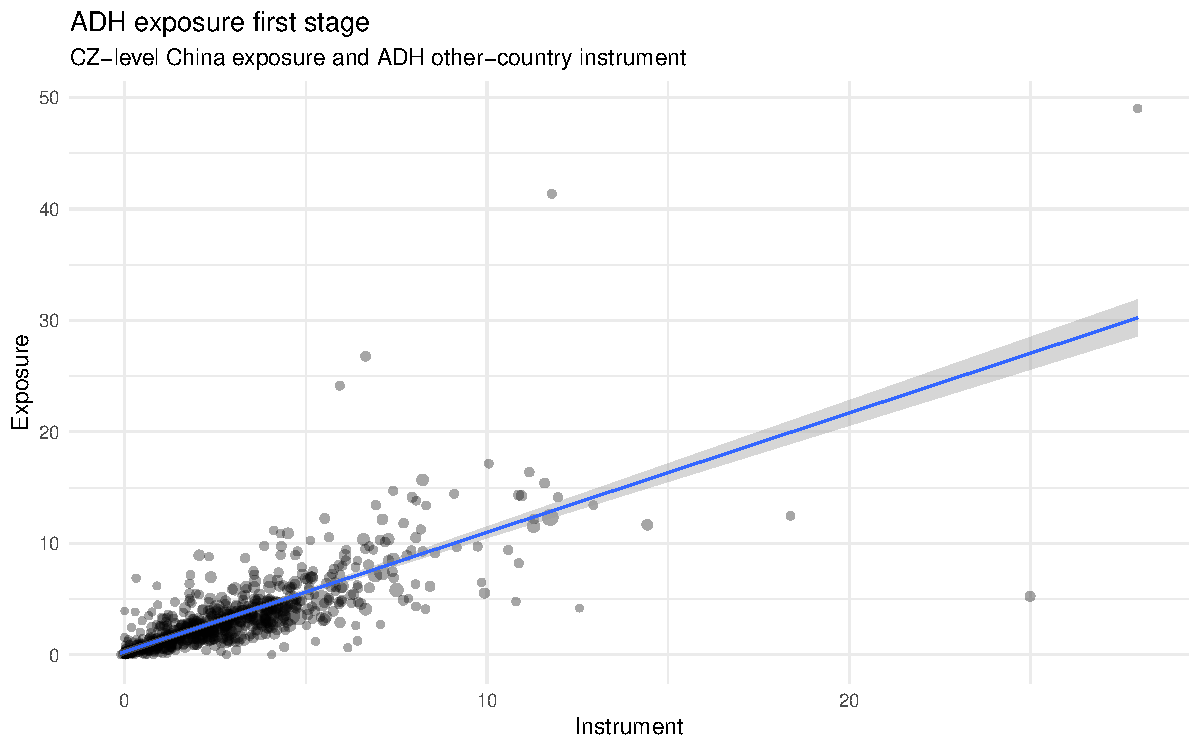
\includegraphics[width=0.85\linewidth,height=\textheight,keepaspectratio]{../output/figures/fig_bartik_first_stage.pdf}

}

\caption{\label{fig-bartik-firststage}First-stage relationship between
ADH exposure and the ADH instrument.}

\end{figure}%

{

\begin{longtable}[]{@{}
  >{\raggedright\arraybackslash}p{(\linewidth - 8\tabcolsep) * \real{0.2222}}
  >{\raggedright\arraybackslash}p{(\linewidth - 8\tabcolsep) * \real{0.2469}}
  >{\raggedright\arraybackslash}p{(\linewidth - 8\tabcolsep) * \real{0.2716}}
  >{\raggedright\arraybackslash}p{(\linewidth - 8\tabcolsep) * \real{0.1728}}
  >{\raggedright\arraybackslash}p{(\linewidth - 8\tabcolsep) * \real{0.0864}}@{}}

\caption{\label{tbl-balance-correlations}Baseline balance: correlations
with exposure and instrument.}

\tabularnewline

\toprule\noalign{}
\begin{minipage}[b]{\linewidth}\raggedright
Variable
\end{minipage} & \begin{minipage}[b]{\linewidth}\raggedright
Corr. with exposure
\end{minipage} & \begin{minipage}[b]{\linewidth}\raggedright
Corr. with instrument
\end{minipage} & \begin{minipage}[b]{\linewidth}\raggedright
Weighted mean
\end{minipage} & \begin{minipage}[b]{\linewidth}\raggedright
SD
\end{minipage} \\
\midrule\noalign{}
\endhead
\bottomrule\noalign{}
\endlastfoot
l\_shind\_manuf\_cbp & 0.574 & 0.614 & 20.695 & 12.848 \\
l\_sh\_popedu\_c & -0.243 & -0.287 & 48.021 & 8.574 \\
l\_sh\_popfborn & -0.145 & -0.131 & 10.146 & 4.969 \\
l\_sh\_empl\_f & 0.028 & 0.006 & 63.624 & 6.634 \\
l\_sh\_routine33 & 0.301 & 0.355 & 32.228 & 3.362 \\
l\_task\_outsource & 0.261 & 0.312 & 0.112 & 0.407 \\
statefip & -0.085 & -0.087 & 27.790 & 14.987 \\

\end{longtable}

}

{

\begin{longtable}[]{@{}
  >{\raggedright\arraybackslash}p{(\linewidth - 10\tabcolsep) * \real{0.3226}}
  >{\raggedright\arraybackslash}p{(\linewidth - 10\tabcolsep) * \real{0.1505}}
  >{\raggedright\arraybackslash}p{(\linewidth - 10\tabcolsep) * \real{0.2258}}
  >{\raggedright\arraybackslash}p{(\linewidth - 10\tabcolsep) * \real{0.0968}}
  >{\raggedright\arraybackslash}p{(\linewidth - 10\tabcolsep) * \real{0.1183}}
  >{\raggedright\arraybackslash}p{(\linewidth - 10\tabcolsep) * \real{0.0860}}@{}}

\caption{\label{tbl-pretrend-placebos}Pre-1988 Republican-margin placebo
diagnostics.}

\tabularnewline

\toprule\noalign{}
\begin{minipage}[b]{\linewidth}\raggedright
Outcome
\end{minipage} & \begin{minipage}[b]{\linewidth}\raggedright
Spec
\end{minipage} & \begin{minipage}[b]{\linewidth}\raggedright
Regressor
\end{minipage} & \begin{minipage}[b]{\linewidth}\raggedright
Estimate
\end{minipage} & \begin{minipage}[b]{\linewidth}\raggedright
Std. error
\end{minipage} & \begin{minipage}[b]{\linewidth}\raggedright
p-value
\end{minipage} \\
\midrule\noalign{}
\endhead
\bottomrule\noalign{}
\endlastfoot
pretrend\_slope\_rep\_margin & minimal & exposure\_1990\_2007 & 0.0001 &
0.0002 & 0.601 \\
pretrend\_slope\_rep\_margin & core\_controls & exposure\_1990\_2007 &
-0.0001 & 0.0002 & 0.700 \\
pretrend\_slope\_rep\_margin & full\_controls & exposure\_1990\_2007 &
-0.0001 & 0.0002 & 0.548 \\
pretrend\_slope\_rep\_margin & minimal & instrument\_1990\_2007 & 0.0000
& 0.0002 & 0.976 \\
pretrend\_slope\_rep\_margin & core\_controls & instrument\_1990\_2007 &
-0.0001 & 0.0002 & 0.556 \\
pretrend\_slope\_rep\_margin & full\_controls & instrument\_1990\_2007 &
-0.0002 & 0.0002 & 0.498 \\
pretrend\_change\_first\_to\_last & minimal & exposure\_1990\_2007 &
0.0075 & 0.0062 & 0.236 \\
pretrend\_change\_first\_to\_last & core\_controls &
exposure\_1990\_2007 & -0.0012 & 0.0056 & 0.833 \\
pretrend\_change\_first\_to\_last & full\_controls &
exposure\_1990\_2007 & -0.0018 & 0.0061 & 0.769 \\
pretrend\_change\_first\_to\_last & minimal & instrument\_1990\_2007 &
0.0064 & 0.0083 & 0.445 \\
pretrend\_change\_first\_to\_last & core\_controls &
instrument\_1990\_2007 & -0.0001 & 0.0081 & 0.990 \\
pretrend\_change\_first\_to\_last & full\_controls &
instrument\_1990\_2007 & -0.0004 & 0.0087 & 0.959 \\

\end{longtable}

}

{

\begin{longtable}[]{@{}
  >{\raggedright\arraybackslash}p{(\linewidth - 12\tabcolsep) * \real{0.0946}}
  >{\raggedright\arraybackslash}p{(\linewidth - 12\tabcolsep) * \real{0.1351}}
  >{\raggedright\arraybackslash}p{(\linewidth - 12\tabcolsep) * \real{0.1216}}
  >{\raggedleft\arraybackslash}p{(\linewidth - 12\tabcolsep) * \real{0.1081}}
  >{\raggedleft\arraybackslash}p{(\linewidth - 12\tabcolsep) * \real{0.1892}}
  >{\raggedleft\arraybackslash}p{(\linewidth - 12\tabcolsep) * \real{0.1622}}
  >{\raggedleft\arraybackslash}p{(\linewidth - 12\tabcolsep) * \real{0.1892}}@{}}

\caption{\label{tbl-industry-shifts}Industry-shift summary from ADH
trade data diagnostics.}

\tabularnewline

\toprule\noalign{}
\begin{minipage}[b]{\linewidth}\raggedright
status
\end{minipage} & \begin{minipage}[b]{\linewidth}\raggedright
period
\end{minipage} & \begin{minipage}[b]{\linewidth}\raggedright
importer
\end{minipage} & \begin{minipage}[b]{\linewidth}\raggedleft
sic87dd
\end{minipage} & \begin{minipage}[b]{\linewidth}\raggedleft
start\_imports
\end{minipage} & \begin{minipage}[b]{\linewidth}\raggedleft
end\_imports
\end{minipage} & \begin{minipage}[b]{\linewidth}\raggedleft
import\_growth
\end{minipage} \\
\midrule\noalign{}
\endhead
\bottomrule\noalign{}
\endlastfoot
ok & 1991-1999 & OTH & 3679 & 143699.73 & 2505878.0 & 2362178.3 \\
ok & 1991-1999 & OTH & 3577 & 40964.04 & 1565398.4 & 1524434.3 \\
ok & 1991-1999 & OTH & 3944 & 1285590.75 & 2732429.2 & 1446838.5 \\
ok & 1991-1999 & OTH & 3651 & 936563.69 & 2377214.8 & 1440651.1 \\
ok & 1991-1999 & OTH & 3861 & 58608.05 & 1004058.8 & 945450.8 \\
ok & 1991-1999 & OTH & 2369 & 1191708.38 & 2126562.8 & 934854.4 \\
ok & 1991-1999 & OTH & 2337 & 1214870.88 & 2095917.0 & 881046.1 \\
ok & 1991-1999 & OTH & 2091 & 235925.19 & 1114860.0 & 878934.8 \\
ok & 1991-1999 & OTH & 3161 & 623382.12 & 1466893.6 & 843511.5 \\
ok & 1991-1999 & OTH & 3089 & 256498.66 & 1082972.6 & 826474.0 \\
ok & 1991-1999 & OTH & 2325 & 634508.31 & 1300735.5 & 666227.2 \\
ok & 1991-1999 & OTH & 2392 & 605945.94 & 1227629.4 & 621683.4 \\
ok & 1991-1999 & OTH & 3021 & 374964.75 & 990012.8 & 615048.1 \\
ok & 1991-1999 & OTH & 2331 & 934854.62 & 1546733.8 & 611879.1 \\
ok & 1991-1999 & OTH & 3357 & 65468.17 & 666530.7 & 601062.5 \\

\end{longtable}

}

\section{Appendix D: Subperiod Exposure and Dynamic
Interpretation}\label{appendix-d-subperiod-exposure-and-dynamic-interpretation}

\begin{figure}[H]

\centering{

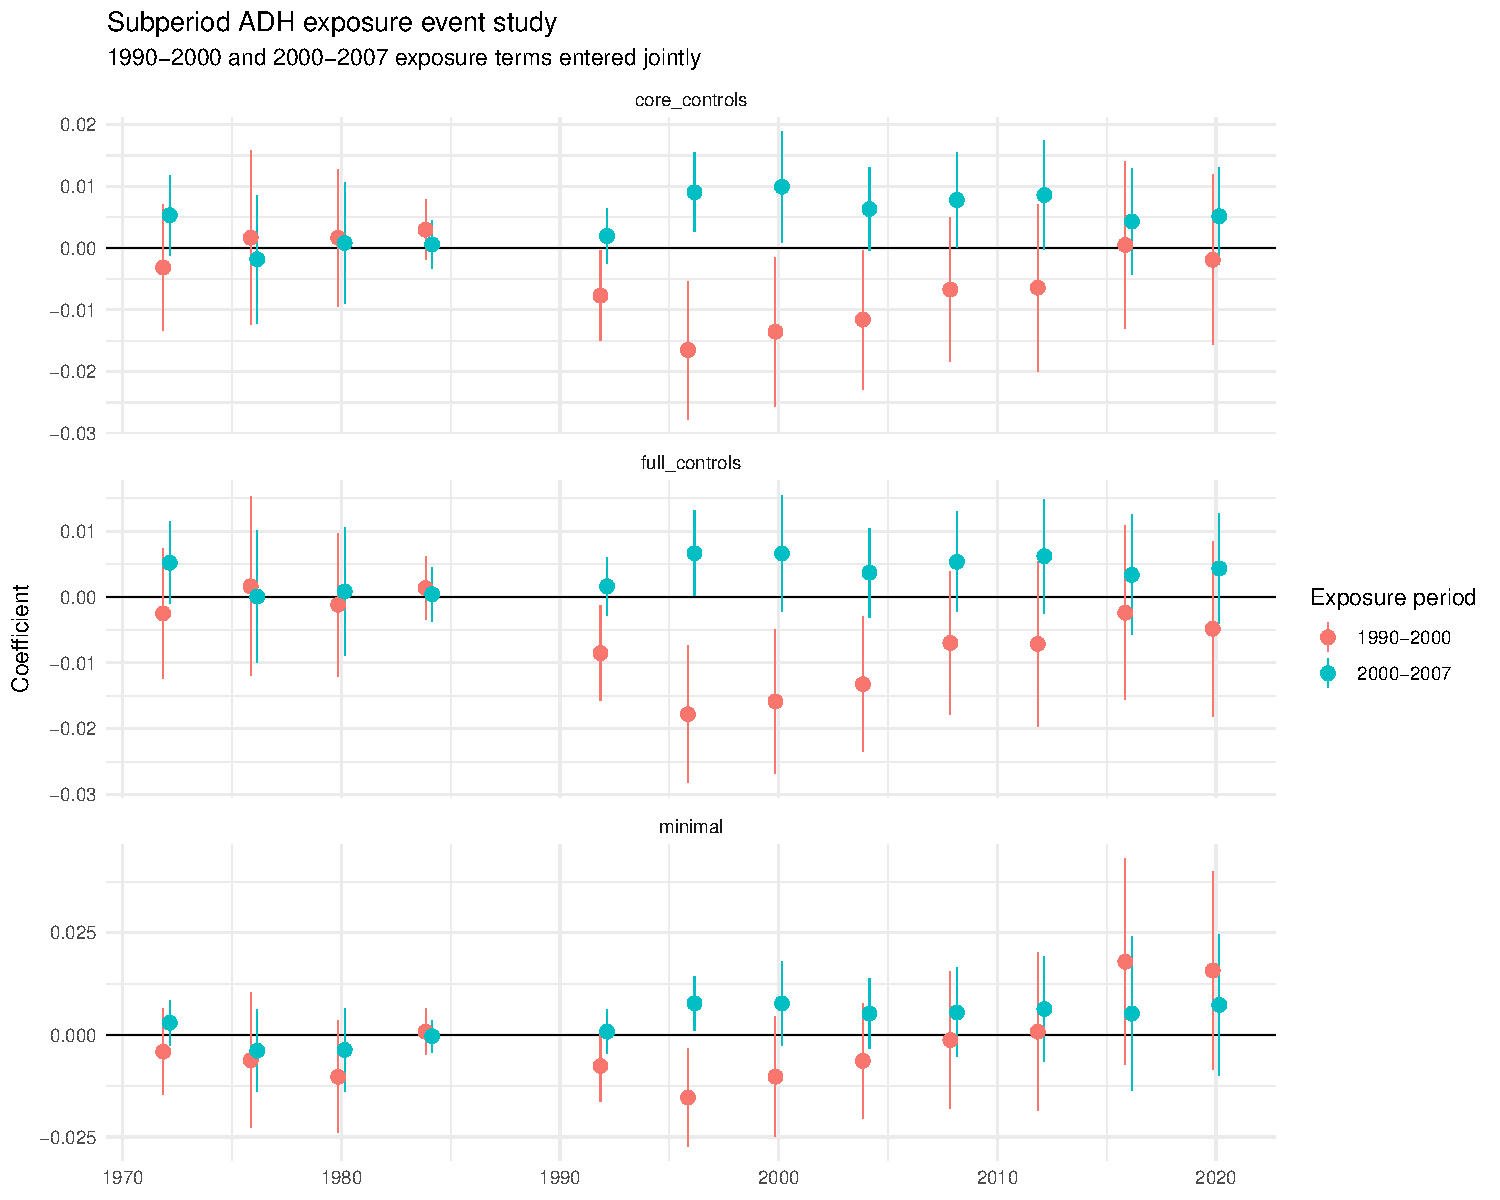
\includegraphics[width=1\linewidth,height=\textheight,keepaspectratio]{../output/figures/fig_subperiod_exposure_event_study.pdf}

}

\caption{\label{fig-subperiod-appendix}Subperiod exposure event-study
estimates.}

\end{figure}%

{

\begin{longtable}[]{@{}
  >{\raggedright\arraybackslash}p{(\linewidth - 10\tabcolsep) * \real{0.1522}}
  >{\raggedleft\arraybackslash}p{(\linewidth - 10\tabcolsep) * \real{0.0543}}
  >{\raggedright\arraybackslash}p{(\linewidth - 10\tabcolsep) * \real{0.2174}}
  >{\raggedright\arraybackslash}p{(\linewidth - 10\tabcolsep) * \real{0.2174}}
  >{\raggedright\arraybackslash}p{(\linewidth - 10\tabcolsep) * \real{0.1848}}
  >{\raggedright\arraybackslash}p{(\linewidth - 10\tabcolsep) * \real{0.1739}}@{}}

\caption{\label{tbl-subperiod-horizons}Selected horizons: early versus
late ADH exposure.}

\tabularnewline

\toprule\noalign{}
\begin{minipage}[b]{\linewidth}\raggedright
Spec
\end{minipage} & \begin{minipage}[b]{\linewidth}\raggedleft
Year
\end{minipage} & \begin{minipage}[b]{\linewidth}\raggedright
1990--2000 exposure
\end{minipage} & \begin{minipage}[b]{\linewidth}\raggedright
2000--2007 exposure
\end{minipage} & \begin{minipage}[b]{\linewidth}\raggedright
Early minus late
\end{minipage} & \begin{minipage}[b]{\linewidth}\raggedright
Approx. p-value
\end{minipage} \\
\midrule\noalign{}
\endhead
\bottomrule\noalign{}
\endlastfoot
Minimal & 1996 & -0.0153 & 0.0077 & -0.0231 & 0.001 \\
Minimal & 2000 & -0.0102 & 0.0077 & -0.0179 & 0.050 \\
Minimal & 2008 & -0.0013 & 0.0055 & -0.0068 & 0.508 \\
Minimal & 2016 & 0.0179 & 0.0052 & 0.0127 & 0.429 \\
Minimal & 2020 & 0.0157 & 0.0073 & 0.0084 & 0.579 \\
Core controls & 1996 & -0.0165 & 0.0090 & -0.0256 & 0.000 \\
Core controls & 2000 & -0.0135 & 0.0099 & -0.0235 & 0.002 \\
Core controls & 2008 & -0.0067 & 0.0078 & -0.0145 & 0.042 \\
Core controls & 2016 & 0.0005 & 0.0043 & -0.0038 & 0.642 \\
Core controls & 2020 & -0.0019 & 0.0052 & -0.0071 & 0.381 \\
Full controls & 1996 & -0.0178 & 0.0067 & -0.0245 & 0.000 \\
Full controls & 2000 & -0.0159 & 0.0066 & -0.0225 & 0.002 \\
Full controls & 2008 & -0.0070 & 0.0053 & -0.0123 & 0.070 \\
Full controls & 2016 & -0.0024 & 0.0034 & -0.0058 & 0.482 \\
Full controls & 2020 & -0.0048 & 0.0043 & -0.0092 & 0.252 \\

\end{longtable}

}

\section{Appendix E: Standard-Error
Diagnostics}\label{appendix-e-standard-error-diagnostics}

{

\begin{longtable}[]{@{}
  >{\raggedright\arraybackslash}p{(\linewidth - 18\tabcolsep) * \real{0.0982}}
  >{\raggedright\arraybackslash}p{(\linewidth - 18\tabcolsep) * \real{0.2455}}
  >{\raggedright\arraybackslash}p{(\linewidth - 18\tabcolsep) * \real{0.0893}}
  >{\raggedright\arraybackslash}p{(\linewidth - 18\tabcolsep) * \real{0.0714}}
  >{\raggedright\arraybackslash}p{(\linewidth - 18\tabcolsep) * \real{0.0938}}
  >{\raggedright\arraybackslash}p{(\linewidth - 18\tabcolsep) * \real{0.0714}}
  >{\raggedright\arraybackslash}p{(\linewidth - 18\tabcolsep) * \real{0.0625}}
  >{\raggedleft\arraybackslash}p{(\linewidth - 18\tabcolsep) * \real{0.0670}}
  >{\raggedleft\arraybackslash}p{(\linewidth - 18\tabcolsep) * \real{0.1027}}
  >{\raggedleft\arraybackslash}p{(\linewidth - 18\tabcolsep) * \real{0.0982}}@{}}

\caption{\label{tbl-vcov-diagnostics}Variance-covariance diagnostics by
specification and SE type.}

\tabularnewline

\toprule\noalign{}
\begin{minipage}[b]{\linewidth}\raggedright
sample
\end{minipage} & \begin{minipage}[b]{\linewidth}\raggedright
spec
\end{minipage} & \begin{minipage}[b]{\linewidth}\raggedright
se\_type
\end{minipage} & \begin{minipage}[b]{\linewidth}\raggedright
status
\end{minipage} & \begin{minipage}[b]{\linewidth}\raggedright
vcov\_repair\_required
\end{minipage} & \begin{minipage}[b]{\linewidth}\raggedright
repair\_required
\end{minipage} & \begin{minipage}[b]{\linewidth}\raggedright
vcov\_repaired
\end{minipage} & \begin{minipage}[b]{\linewidth}\raggedleft
min\_eigenvalue
\end{minipage} & \begin{minipage}[b]{\linewidth}\raggedleft
n\_negative\_eigenvalues
\end{minipage} & \begin{minipage}[b]{\linewidth}\raggedleft
max\_abs\_repair\_change
\end{minipage} \\
\midrule\noalign{}
\endhead
\bottomrule\noalign{}
\endlastfoot
main\_1972\_start & minimal\_full\_panel & heteroskedastic & ok & FALSE
& FALSE & FALSE & 0.0000022 & 0 & NA \\
main\_1972\_start & minimal\_full\_panel & cluster\_cz & ok & FALSE &
FALSE & FALSE & 0.0000001 & 0 & NA \\
main\_1972\_start & minimal\_full\_panel & cluster\_state & ok & FALSE &
FALSE & FALSE & 0.0000001 & 0 & NA \\
main\_1972\_start & minimal\_full\_panel & cluster\_cz\_year &
repair\_required & TRUE & TRUE & FALSE & -0.0000403 & 10 & NA \\
main\_1972\_start & minimal\_full\_panel & newey\_west\_lag1 & ok &
FALSE & FALSE & FALSE & 0.0000012 & 0 & NA \\
main\_1972\_start & minimal\_full\_panel & driscoll\_kraay\_lag1 & ok &
FALSE & FALSE & FALSE & 0.0000000 & 0 & NA \\
main\_1972\_start & minimal\_full\_panel & conley\_250km & ok & FALSE &
FALSE & FALSE & 0.0000001 & 0 & NA \\
main\_1972\_start & minimal\_full\_panel & conley\_500km &
repair\_required & TRUE & TRUE & FALSE & -0.0000057 & 2 & NA \\
main\_1972\_start & minimal\_full\_panel & conley\_750km &
repair\_required & TRUE & TRUE & FALSE & -0.0000041 & 4 & NA \\
main\_1972\_start & minimal\_full\_panel & conley\_1000km &
repair\_required & TRUE & TRUE & FALSE & -0.0000073 & 4 & NA \\
main\_1972\_start & interacted\_core\_controls\_diagnostic &
heteroskedastic & ok & FALSE & FALSE & FALSE & 0.0000011 & 0 & NA \\
main\_1972\_start & interacted\_core\_controls\_diagnostic & cluster\_cz
& ok & FALSE & FALSE & FALSE & 0.0000000 & 0 & NA \\
main\_1972\_start & interacted\_core\_controls\_diagnostic &
cluster\_state & ok & FALSE & FALSE & FALSE & 0.0000000 & 1 & NA \\
main\_1972\_start & interacted\_core\_controls\_diagnostic &
cluster\_cz\_year & repair\_required & TRUE & TRUE & FALSE & -0.0004383
& 35 & NA \\
main\_1972\_start & interacted\_core\_controls\_diagnostic &
newey\_west\_lag1 & ok & FALSE & FALSE & FALSE & 0.0000006 & 0 & NA \\
main\_1972\_start & interacted\_core\_controls\_diagnostic &
driscoll\_kraay\_lag1 & ok & FALSE & FALSE & FALSE & 0.0000000 & 17 &
NA \\
main\_1972\_start & interacted\_core\_controls\_diagnostic &
conley\_250km & repair\_required & TRUE & TRUE & FALSE & -0.0000107 & 7
& NA \\
main\_1972\_start & interacted\_core\_controls\_diagnostic &
conley\_500km & repair\_required & TRUE & TRUE & FALSE & -0.0000835 & 18
& NA \\
main\_1972\_start & interacted\_core\_controls\_diagnostic &
conley\_750km & repair\_required & TRUE & TRUE & FALSE & -0.0001852 & 21
& NA \\
main\_1972\_start & interacted\_core\_controls\_diagnostic &
conley\_1000km & repair\_required & TRUE & TRUE & FALSE & -0.0003335 &
22 & NA \\
main\_1972\_start & interacted\_controls\_full\_panel & heteroskedastic
& ok & FALSE & FALSE & FALSE & 0.0000010 & 0 & NA \\
main\_1972\_start & interacted\_controls\_full\_panel & cluster\_cz & ok
& FALSE & FALSE & FALSE & 0.0000000 & 0 & NA \\
main\_1972\_start & interacted\_controls\_full\_panel & cluster\_state &
ok & FALSE & FALSE & FALSE & 0.0000000 & 18 & NA \\
main\_1972\_start & interacted\_controls\_full\_panel &
cluster\_cz\_year & repair\_required & TRUE & TRUE & FALSE & -0.0006599
& 63 & NA \\
main\_1972\_start & interacted\_controls\_full\_panel &
newey\_west\_lag1 & ok & FALSE & FALSE & FALSE & 0.0000006 & 0 & NA \\
main\_1972\_start & interacted\_controls\_full\_panel &
driscoll\_kraay\_lag1 & ok & FALSE & FALSE & FALSE & 0.0000000 & 35 &
NA \\
main\_1972\_start & interacted\_controls\_full\_panel & conley\_250km &
repair\_required & TRUE & TRUE & FALSE & -0.0000974 & 24 & NA \\
main\_1972\_start & interacted\_controls\_full\_panel & conley\_500km &
repair\_required & TRUE & TRUE & FALSE & -0.0007051 & 36 & NA \\
main\_1972\_start & interacted\_controls\_full\_panel & conley\_750km &
repair\_required & TRUE & TRUE & FALSE & -0.0011557 & 40 & NA \\
main\_1972\_start & interacted\_controls\_full\_panel & conley\_1000km &
repair\_required & TRUE & TRUE & FALSE & -0.0019790 & 40 & NA \\
main\_1972\_start &
interacted\_controls\_full\_panel\_raw\_controls\_diagnostic &
heteroskedastic & ok & FALSE & FALSE & FALSE & 0.0000001 & 0 & NA \\
main\_1972\_start &
interacted\_controls\_full\_panel\_raw\_controls\_diagnostic &
cluster\_cz & ok & FALSE & FALSE & FALSE & 0.0000000 & 0 & NA \\
main\_1972\_start &
interacted\_controls\_full\_panel\_raw\_controls\_diagnostic &
cluster\_state & ok & FALSE & FALSE & FALSE & 0.0000000 & 20 & NA \\
main\_1972\_start &
interacted\_controls\_full\_panel\_raw\_controls\_diagnostic &
cluster\_cz\_year & repair\_required & TRUE & TRUE & FALSE & -0.0019361
& 63 & NA \\
main\_1972\_start &
interacted\_controls\_full\_panel\_raw\_controls\_diagnostic &
newey\_west\_lag1 & ok & FALSE & FALSE & FALSE & 0.0000000 & 0 & NA \\
main\_1972\_start &
interacted\_controls\_full\_panel\_raw\_controls\_diagnostic &
driscoll\_kraay\_lag1 & ok & FALSE & FALSE & FALSE & 0.0000000 & 35 &
NA \\
main\_1972\_start &
interacted\_controls\_full\_panel\_raw\_controls\_diagnostic &
conley\_250km & repair\_required & TRUE & TRUE & FALSE & -0.0000139 & 24
& NA \\
main\_1972\_start &
interacted\_controls\_full\_panel\_raw\_controls\_diagnostic &
conley\_500km & repair\_required & TRUE & TRUE & FALSE & -0.0007107 & 36
& NA \\
main\_1972\_start &
interacted\_controls\_full\_panel\_raw\_controls\_diagnostic &
conley\_750km & repair\_required & TRUE & TRUE & FALSE & -0.0003939 & 40
& NA \\
main\_1972\_start &
interacted\_controls\_full\_panel\_raw\_controls\_diagnostic &
conley\_1000km & repair\_required & TRUE & TRUE & FALSE & -0.0028599 &
40 & NA \\
diagnostic\_1952\_start & minimal\_full\_panel & heteroskedastic & ok &
FALSE & FALSE & FALSE & 0.0000020 & 0 & NA \\
diagnostic\_1952\_start & minimal\_full\_panel & cluster\_cz & ok &
FALSE & FALSE & FALSE & 0.0000001 & 0 & NA \\
diagnostic\_1952\_start & minimal\_full\_panel & cluster\_state & ok &
FALSE & FALSE & FALSE & 0.0000000 & 0 & NA \\
diagnostic\_1952\_start & minimal\_full\_panel & cluster\_cz\_year &
repair\_required & TRUE & TRUE & FALSE & -0.0000385 & 14 & NA \\
diagnostic\_1952\_start & minimal\_full\_panel & newey\_west\_lag1 & ok
& FALSE & FALSE & FALSE & 0.0000014 & 0 & NA \\
diagnostic\_1952\_start & minimal\_full\_panel & driscoll\_kraay\_lag1 &
ok & FALSE & FALSE & FALSE & 0.0000000 & 0 & NA \\
diagnostic\_1952\_start & minimal\_full\_panel & conley\_250km &
repair\_required & TRUE & TRUE & FALSE & -0.0000001 & 1 & NA \\
diagnostic\_1952\_start & minimal\_full\_panel & conley\_500km &
repair\_required & TRUE & TRUE & FALSE & -0.0000112 & 4 & NA \\
diagnostic\_1952\_start & minimal\_full\_panel & conley\_750km &
repair\_required & TRUE & TRUE & FALSE & -0.0000233 & 7 & NA \\
diagnostic\_1952\_start & minimal\_full\_panel & conley\_1000km &
repair\_required & TRUE & TRUE & FALSE & -0.0000152 & 7 & NA \\
diagnostic\_1952\_start & interacted\_core\_controls\_diagnostic &
heteroskedastic & ok & FALSE & FALSE & FALSE & 0.0000014 & 0 & NA \\
diagnostic\_1952\_start & interacted\_core\_controls\_diagnostic &
cluster\_cz & ok & FALSE & FALSE & FALSE & 0.0000000 & 0 & NA \\
diagnostic\_1952\_start & interacted\_core\_controls\_diagnostic &
cluster\_state & ok & FALSE & FALSE & FALSE & 0.0000000 & 10 & NA \\
diagnostic\_1952\_start & interacted\_core\_controls\_diagnostic &
cluster\_cz\_year & repair\_required & TRUE & TRUE & FALSE & -0.0004952
& 53 & NA \\
diagnostic\_1952\_start & interacted\_core\_controls\_diagnostic &
newey\_west\_lag1 & ok & FALSE & FALSE & FALSE & 0.0000007 & 0 & NA \\
diagnostic\_1952\_start & interacted\_core\_controls\_diagnostic &
driscoll\_kraay\_lag1 & ok & FALSE & FALSE & FALSE & 0.0000000 & 25 &
NA \\
diagnostic\_1952\_start & interacted\_core\_controls\_diagnostic &
conley\_250km & repair\_required & TRUE & TRUE & FALSE & -0.0000240 & 16
& NA \\
diagnostic\_1952\_start & interacted\_core\_controls\_diagnostic &
conley\_500km & repair\_required & TRUE & TRUE & FALSE & -0.0002296 & 28
& NA \\
diagnostic\_1952\_start & interacted\_core\_controls\_diagnostic &
conley\_750km & repair\_required & TRUE & TRUE & FALSE & -0.0004917 & 31
& NA \\
diagnostic\_1952\_start & interacted\_core\_controls\_diagnostic &
conley\_1000km & repair\_required & TRUE & TRUE & FALSE & -0.0010091 &
33 & NA \\
diagnostic\_1952\_start & interacted\_controls\_full\_panel &
heteroskedastic & ok & FALSE & FALSE & FALSE & 0.0000011 & 0 & NA \\
diagnostic\_1952\_start & interacted\_controls\_full\_panel &
cluster\_cz & ok & FALSE & FALSE & FALSE & 0.0000000 & 0 & NA \\
diagnostic\_1952\_start & interacted\_controls\_full\_panel &
cluster\_state & ok & FALSE & FALSE & FALSE & 0.0000000 & 36 & NA \\
diagnostic\_1952\_start & interacted\_controls\_full\_panel &
cluster\_cz\_year & repair\_required & TRUE & TRUE & FALSE & -0.0011482
& 94 & NA \\
diagnostic\_1952\_start & interacted\_controls\_full\_panel &
newey\_west\_lag1 & ok & FALSE & FALSE & FALSE & 0.0000006 & 0 & NA \\
diagnostic\_1952\_start & interacted\_controls\_full\_panel &
driscoll\_kraay\_lag1 & ok & FALSE & FALSE & FALSE & 0.0000000 & 50 &
NA \\
diagnostic\_1952\_start & interacted\_controls\_full\_panel &
conley\_250km & repair\_required & TRUE & TRUE & FALSE & -0.0002214 & 39
& NA \\
diagnostic\_1952\_start & interacted\_controls\_full\_panel &
conley\_500km & repair\_required & TRUE & TRUE & FALSE & -0.0012160 & 54
& NA \\
diagnostic\_1952\_start & interacted\_controls\_full\_panel &
conley\_750km & repair\_required & TRUE & TRUE & FALSE & -0.0025146 & 56
& NA \\
diagnostic\_1952\_start & interacted\_controls\_full\_panel &
conley\_1000km & repair\_required & TRUE & TRUE & FALSE & -0.0040057 &
57 & NA \\
diagnostic\_1952\_start &
interacted\_controls\_full\_panel\_raw\_controls\_diagnostic &
heteroskedastic & ok & FALSE & FALSE & FALSE & 0.0000001 & 0 & NA \\
diagnostic\_1952\_start &
interacted\_controls\_full\_panel\_raw\_controls\_diagnostic &
cluster\_cz & ok & FALSE & FALSE & FALSE & 0.0000000 & 0 & NA \\
diagnostic\_1952\_start &
interacted\_controls\_full\_panel\_raw\_controls\_diagnostic &
cluster\_state & ok & FALSE & FALSE & FALSE & 0.0000000 & 37 & NA \\
diagnostic\_1952\_start &
interacted\_controls\_full\_panel\_raw\_controls\_diagnostic &
cluster\_cz\_year & repair\_required & TRUE & TRUE & FALSE & -0.0040369
& 94 & NA \\
diagnostic\_1952\_start &
interacted\_controls\_full\_panel\_raw\_controls\_diagnostic &
newey\_west\_lag1 & ok & FALSE & FALSE & FALSE & 0.0000000 & 0 & NA \\
diagnostic\_1952\_start &
interacted\_controls\_full\_panel\_raw\_controls\_diagnostic &
driscoll\_kraay\_lag1 & ok & FALSE & FALSE & FALSE & 0.0000000 & 51 &
NA \\
diagnostic\_1952\_start &
interacted\_controls\_full\_panel\_raw\_controls\_diagnostic &
conley\_250km & repair\_required & TRUE & TRUE & FALSE & -0.0000431 & 39
& NA \\
diagnostic\_1952\_start &
interacted\_controls\_full\_panel\_raw\_controls\_diagnostic &
conley\_500km & repair\_required & TRUE & TRUE & FALSE & -0.0011073 & 54
& NA \\
diagnostic\_1952\_start &
interacted\_controls\_full\_panel\_raw\_controls\_diagnostic &
conley\_750km & repair\_required & TRUE & TRUE & FALSE & -0.0009977 & 56
& NA \\
diagnostic\_1952\_start &
interacted\_controls\_full\_panel\_raw\_controls\_diagnostic &
conley\_1000km & repair\_required & TRUE & TRUE & FALSE & -0.0055161 &
57 & NA \\

\end{longtable}

}

{

\begin{longtable}[]{@{}
  >{\raggedright\arraybackslash}p{(\linewidth - 32\tabcolsep) * \real{0.0514}}
  >{\raggedright\arraybackslash}p{(\linewidth - 32\tabcolsep) * \real{0.1285}}
  >{\raggedright\arraybackslash}p{(\linewidth - 32\tabcolsep) * \real{0.0467}}
  >{\raggedleft\arraybackslash}p{(\linewidth - 32\tabcolsep) * \real{0.0491}}
  >{\raggedleft\arraybackslash}p{(\linewidth - 32\tabcolsep) * \real{0.0327}}
  >{\raggedleft\arraybackslash}p{(\linewidth - 32\tabcolsep) * \real{0.0397}}
  >{\raggedleft\arraybackslash}p{(\linewidth - 32\tabcolsep) * \real{0.0327}}
  >{\raggedleft\arraybackslash}p{(\linewidth - 32\tabcolsep) * \real{0.0444}}
  >{\raggedleft\arraybackslash}p{(\linewidth - 32\tabcolsep) * \real{0.0444}}
  >{\raggedleft\arraybackslash}p{(\linewidth - 32\tabcolsep) * \real{0.0210}}
  >{\raggedleft\arraybackslash}p{(\linewidth - 32\tabcolsep) * \real{0.0234}}
  >{\raggedleft\arraybackslash}p{(\linewidth - 32\tabcolsep) * \real{0.0491}}
  >{\raggedright\arraybackslash}p{(\linewidth - 32\tabcolsep) * \real{0.0374}}
  >{\raggedright\arraybackslash}p{(\linewidth - 32\tabcolsep) * \real{0.0374}}
  >{\raggedright\arraybackslash}p{(\linewidth - 32\tabcolsep) * \real{0.0327}}
  >{\raggedleft\arraybackslash}p{(\linewidth - 32\tabcolsep) * \real{0.0350}}
  >{\raggedright\arraybackslash}p{(\linewidth - 32\tabcolsep) * \real{0.2944}}@{}}

\caption{\label{tbl-se-warning-diagnostics}SE warning diagnostics.}

\tabularnewline

\toprule\noalign{}
\begin{minipage}[b]{\linewidth}\raggedright
sample
\end{minipage} & \begin{minipage}[b]{\linewidth}\raggedright
spec
\end{minipage} & \begin{minipage}[b]{\linewidth}\raggedright
se\_type
\end{minipage} & \begin{minipage}[b]{\linewidth}\raggedleft
n\_event\_coefficients
\end{minipage} & \begin{minipage}[b]{\linewidth}\raggedleft
min\_std\_error
\end{minipage} & \begin{minipage}[b]{\linewidth}\raggedleft
median\_std\_error
\end{minipage} & \begin{minipage}[b]{\linewidth}\raggedleft
max\_std\_error
\end{minipage} & \begin{minipage}[b]{\linewidth}\raggedleft
near\_zero\_se\_count
\end{minipage} & \begin{minipage}[b]{\linewidth}\raggedleft
nonfinite\_se\_count
\end{minipage} & \begin{minipage}[b]{\linewidth}\raggedleft
vcov\_dim
\end{minipage} & \begin{minipage}[b]{\linewidth}\raggedleft
vcov\_rank
\end{minipage} & \begin{minipage}[b]{\linewidth}\raggedleft
vcov\_rank\_deficiency
\end{minipage} & \begin{minipage}[b]{\linewidth}\raggedright
vcov\_status
\end{minipage} & \begin{minipage}[b]{\linewidth}\raggedright
repair\_required
\end{minipage} & \begin{minipage}[b]{\linewidth}\raggedright
vcov\_repaired
\end{minipage} & \begin{minipage}[b]{\linewidth}\raggedleft
min\_eigenvalue
\end{minipage} & \begin{minipage}[b]{\linewidth}\raggedright
diagnostic\_note
\end{minipage} \\
\midrule\noalign{}
\endhead
\bottomrule\noalign{}
\endlastfoot
diagnostic\_1952\_start & interacted\_controls\_full\_panel &
cluster\_cz & 17 & 0.0011450 & 0.0028558 & 0.0055053 & 0 & 0 & 119 & 119
& 0 & ok & FALSE & FALSE & 0.0000000 & NA \\
diagnostic\_1952\_start & interacted\_controls\_full\_panel &
cluster\_cz\_year & 17 & 0.0003398 & 0.0012840 & 0.0020663 & 0 & 8 & 119
& 119 & 0 & repair\_required & TRUE & FALSE & -0.0011482 & Two-way
clustering includes very few year clusters; use as diagnostic only. \\
diagnostic\_1952\_start & interacted\_controls\_full\_panel &
cluster\_state & 17 & 0.0012618 & 0.0031569 & 0.0071144 & 0 & 0 & 119 &
47 & 72 & ok & FALSE & FALSE & 0.0000000 & VCOV is rank deficient; use
as diagnostic only unless justified. \\
diagnostic\_1952\_start & interacted\_controls\_full\_panel &
conley\_1000km & 17 & 0.0010730 & 0.0039122 & 0.0071460 & 0 & 1 & 119 &
119 & 0 & repair\_required & TRUE & FALSE & -0.0040057 & Conley VCOV is
non-positive-definite before repair or requires numerical repair;
diagnostic only unless separately justified. \\
diagnostic\_1952\_start & interacted\_controls\_full\_panel &
conley\_250km & 17 & 0.0013422 & 0.0035539 & 0.0080085 & 0 & 0 & 119 &
119 & 0 & repair\_required & TRUE & FALSE & -0.0002214 & Conley VCOV is
non-positive-definite before repair or requires numerical repair;
diagnostic only unless separately justified. \\
diagnostic\_1952\_start & interacted\_controls\_full\_panel &
conley\_500km & 17 & 0.0012428 & 0.0037343 & 0.0092022 & 0 & 0 & 119 &
119 & 0 & repair\_required & TRUE & FALSE & -0.0012160 & Conley VCOV is
non-positive-definite before repair or requires numerical repair;
diagnostic only unless separately justified. \\
diagnostic\_1952\_start & interacted\_controls\_full\_panel &
conley\_750km & 17 & 0.0011858 & 0.0040711 & 0.0058539 & 0 & 1 & 119 &
119 & 0 & repair\_required & TRUE & FALSE & -0.0025146 & Conley VCOV is
non-positive-definite before repair or requires numerical repair;
diagnostic only unless separately justified. \\
diagnostic\_1952\_start & interacted\_controls\_full\_panel &
driscoll\_kraay\_lag1 & 17 & 0.0000000 & 0.0000000 & 0.0000000 & 17 & 0
& 119 & 51 & 68 & ok & FALSE & FALSE & 0.0000000 & Suspicious near-zero
Driscoll-Kraay SEs and rank-deficient VCOV; do not report without
further diagnosis. \\
diagnostic\_1952\_start & interacted\_controls\_full\_panel &
heteroskedastic & 17 & 0.0021333 & 0.0029210 & 0.0053774 & 0 & 0 & 119 &
119 & 0 & ok & FALSE & FALSE & 0.0000011 & NA \\
diagnostic\_1952\_start & interacted\_controls\_full\_panel &
newey\_west\_lag1 & 17 & 0.0017730 & 0.0030056 & 0.0055331 & 0 & 0 & 119
& 119 & 0 & ok & FALSE & FALSE & 0.0000006 & NA \\
diagnostic\_1952\_start &
interacted\_controls\_full\_panel\_raw\_controls\_diagnostic &
cluster\_cz & 17 & 0.0011450 & 0.0028558 & 0.0055053 & 0 & 0 & 119 & 119
& 0 & ok & FALSE & FALSE & 0.0000000 & NA \\
diagnostic\_1952\_start &
interacted\_controls\_full\_panel\_raw\_controls\_diagnostic &
cluster\_cz\_year & 17 & 0.0003398 & 0.0012840 & 0.0020663 & 0 & 8 & 119
& 119 & 0 & repair\_required & TRUE & FALSE & -0.0040369 & Two-way
clustering includes very few year clusters; use as diagnostic only. \\
diagnostic\_1952\_start &
interacted\_controls\_full\_panel\_raw\_controls\_diagnostic &
cluster\_state & 17 & 0.0012618 & 0.0031569 & 0.0071144 & 0 & 0 & 119 &
50 & 69 & ok & FALSE & FALSE & 0.0000000 & VCOV is rank deficient; use
as diagnostic only unless justified. \\
diagnostic\_1952\_start &
interacted\_controls\_full\_panel\_raw\_controls\_diagnostic &
conley\_1000km & 17 & 0.0010730 & 0.0039122 & 0.0071460 & 0 & 1 & 119 &
119 & 0 & repair\_required & TRUE & FALSE & -0.0055161 & Conley VCOV is
non-positive-definite before repair or requires numerical repair;
diagnostic only unless separately justified. \\
diagnostic\_1952\_start &
interacted\_controls\_full\_panel\_raw\_controls\_diagnostic &
conley\_250km & 17 & 0.0013422 & 0.0035539 & 0.0080085 & 0 & 0 & 119 &
119 & 0 & repair\_required & TRUE & FALSE & -0.0000431 & Conley VCOV is
non-positive-definite before repair or requires numerical repair;
diagnostic only unless separately justified. \\
diagnostic\_1952\_start &
interacted\_controls\_full\_panel\_raw\_controls\_diagnostic &
conley\_500km & 17 & 0.0012428 & 0.0037343 & 0.0092022 & 0 & 0 & 119 &
119 & 0 & repair\_required & TRUE & FALSE & -0.0011073 & Conley VCOV is
non-positive-definite before repair or requires numerical repair;
diagnostic only unless separately justified. \\
diagnostic\_1952\_start &
interacted\_controls\_full\_panel\_raw\_controls\_diagnostic &
conley\_750km & 17 & 0.0011858 & 0.0040711 & 0.0058539 & 0 & 1 & 119 &
119 & 0 & repair\_required & TRUE & FALSE & -0.0009977 & Conley VCOV is
non-positive-definite before repair or requires numerical repair;
diagnostic only unless separately justified. \\
diagnostic\_1952\_start &
interacted\_controls\_full\_panel\_raw\_controls\_diagnostic &
driscoll\_kraay\_lag1 & 17 & 0.0000000 & 0.0000000 & 0.0000000 & 17 & 0
& 119 & 63 & 56 & ok & FALSE & FALSE & 0.0000000 & Suspicious near-zero
Driscoll-Kraay SEs and rank-deficient VCOV; do not report without
further diagnosis. \\
diagnostic\_1952\_start &
interacted\_controls\_full\_panel\_raw\_controls\_diagnostic &
heteroskedastic & 17 & 0.0021333 & 0.0029210 & 0.0053774 & 0 & 0 & 119 &
119 & 0 & ok & FALSE & FALSE & 0.0000001 & NA \\
diagnostic\_1952\_start &
interacted\_controls\_full\_panel\_raw\_controls\_diagnostic &
newey\_west\_lag1 & 17 & 0.0017730 & 0.0030056 & 0.0055331 & 0 & 0 & 119
& 119 & 0 & ok & FALSE & FALSE & 0.0000000 & NA \\
diagnostic\_1952\_start & interacted\_core\_controls\_diagnostic &
cluster\_cz & 17 & 0.0011361 & 0.0026991 & 0.0054382 & 0 & 0 & 68 & 68 &
0 & ok & FALSE & FALSE & 0.0000000 & NA \\
diagnostic\_1952\_start & interacted\_core\_controls\_diagnostic &
cluster\_cz\_year & 17 & 0.0007968 & 0.0021135 & 0.0025131 & 0 & 10 & 68
& 68 & 0 & repair\_required & TRUE & FALSE & -0.0004952 & Two-way
clustering includes very few year clusters; use as diagnostic only. \\
diagnostic\_1952\_start & interacted\_core\_controls\_diagnostic &
cluster\_state & 17 & 0.0012829 & 0.0031404 & 0.0065168 & 0 & 0 & 68 &
47 & 21 & ok & FALSE & FALSE & 0.0000000 & VCOV is rank deficient; use
as diagnostic only unless justified. \\
diagnostic\_1952\_start & interacted\_core\_controls\_diagnostic &
conley\_1000km & 17 & 0.0009920 & 0.0033095 & 0.0069653 & 0 & 0 & 68 &
68 & 0 & repair\_required & TRUE & FALSE & -0.0010091 & Conley VCOV is
non-positive-definite before repair or requires numerical repair;
diagnostic only unless separately justified. \\
diagnostic\_1952\_start & interacted\_core\_controls\_diagnostic &
conley\_250km & 17 & 0.0012790 & 0.0035720 & 0.0078193 & 0 & 0 & 68 & 68
& 0 & repair\_required & TRUE & FALSE & -0.0000240 & Conley VCOV is
non-positive-definite before repair or requires numerical repair;
diagnostic only unless separately justified. \\
diagnostic\_1952\_start & interacted\_core\_controls\_diagnostic &
conley\_500km & 17 & 0.0005874 & 0.0036427 & 0.0082181 & 0 & 0 & 68 & 68
& 0 & repair\_required & TRUE & FALSE & -0.0002296 & Conley VCOV is
non-positive-definite before repair or requires numerical repair;
diagnostic only unless separately justified. \\
diagnostic\_1952\_start & interacted\_core\_controls\_diagnostic &
conley\_750km & 17 & 0.0011282 & 0.0038821 & 0.0058691 & 0 & 1 & 68 & 68
& 0 & repair\_required & TRUE & FALSE & -0.0004917 & Conley VCOV is
non-positive-definite before repair or requires numerical repair;
diagnostic only unless separately justified. \\
diagnostic\_1952\_start & interacted\_core\_controls\_diagnostic &
driscoll\_kraay\_lag1 & 17 & 0.0000000 & 0.0000000 & 0.0000000 & 17 & 0
& 68 & 28 & 40 & ok & FALSE & FALSE & 0.0000000 & Suspicious near-zero
Driscoll-Kraay SEs and rank-deficient VCOV; do not report without
further diagnosis. \\
diagnostic\_1952\_start & interacted\_core\_controls\_diagnostic &
heteroskedastic & 17 & 0.0023645 & 0.0029059 & 0.0051776 & 0 & 0 & 68 &
68 & 0 & ok & FALSE & FALSE & 0.0000014 & NA \\
diagnostic\_1952\_start & interacted\_core\_controls\_diagnostic &
newey\_west\_lag1 & 17 & 0.0019190 & 0.0029901 & 0.0053275 & 0 & 0 & 68
& 68 & 0 & ok & FALSE & FALSE & 0.0000007 & NA \\
diagnostic\_1952\_start & minimal\_full\_panel & cluster\_cz & 17 &
0.0012447 & 0.0038491 & 0.0068718 & 0 & 0 & 17 & 17 & 0 & ok & FALSE &
FALSE & 0.0000001 & NA \\
diagnostic\_1952\_start & minimal\_full\_panel & cluster\_cz\_year & 17
& 0.0003390 & 0.0009342 & 0.0022609 & 0 & 7 & 17 & 17 & 0 &
repair\_required & TRUE & FALSE & -0.0000385 & Two-way clustering
includes very few year clusters; use as diagnostic only. \\
diagnostic\_1952\_start & minimal\_full\_panel & cluster\_state & 17 &
0.0016513 & 0.0049190 & 0.0087699 & 0 & 0 & 17 & 17 & 0 & ok & FALSE &
FALSE & 0.0000000 & NA \\
diagnostic\_1952\_start & minimal\_full\_panel & conley\_1000km & 17 &
0.0013982 & 0.0058193 & 0.0125125 & 0 & 0 & 17 & 17 & 0 &
repair\_required & TRUE & FALSE & -0.0000152 & Conley VCOV is
non-positive-definite before repair or requires numerical repair;
diagnostic only unless separately justified. \\
diagnostic\_1952\_start & minimal\_full\_panel & conley\_250km & 17 &
0.0018948 & 0.0051039 & 0.0087177 & 0 & 0 & 17 & 17 & 0 &
repair\_required & TRUE & FALSE & -0.0000001 & Conley VCOV is
non-positive-definite before repair or requires numerical repair;
diagnostic only unless separately justified. \\
diagnostic\_1952\_start & minimal\_full\_panel & conley\_500km & 17 &
0.0019134 & 0.0053149 & 0.0107249 & 0 & 0 & 17 & 17 & 0 &
repair\_required & TRUE & FALSE & -0.0000112 & Conley VCOV is
non-positive-definite before repair or requires numerical repair;
diagnostic only unless separately justified. \\
diagnostic\_1952\_start & minimal\_full\_panel & conley\_750km & 17 &
0.0021888 & 0.0054710 & 0.0114147 & 0 & 0 & 17 & 17 & 0 &
repair\_required & TRUE & FALSE & -0.0000233 & Conley VCOV is
non-positive-definite before repair or requires numerical repair;
diagnostic only unless separately justified. \\
diagnostic\_1952\_start & minimal\_full\_panel & driscoll\_kraay\_lag1 &
17 & 0.0000000 & 0.0000000 & 0.0000000 & 17 & 0 & 17 & 17 & 0 & ok &
FALSE & FALSE & 0.0000000 & Suspicious near-zero Driscoll-Kraay SEs; do
not report without further diagnosis. \\
diagnostic\_1952\_start & minimal\_full\_panel & heteroskedastic & 17 &
0.0020400 & 0.0039947 & 0.0066970 & 0 & 0 & 17 & 17 & 0 & ok & FALSE &
FALSE & 0.0000020 & NA \\
diagnostic\_1952\_start & minimal\_full\_panel & newey\_west\_lag1 & 17
& 0.0017522 & 0.0041104 & 0.0068909 & 0 & 0 & 17 & 17 & 0 & ok & FALSE &
FALSE & 0.0000014 & NA \\
main\_1972\_start & interacted\_controls\_full\_panel & cluster\_cz & 12
& 0.0011449 & 0.0027069 & 0.0032709 & 0 & 0 & 84 & 84 & 0 & ok & FALSE &
FALSE & 0.0000000 & NA \\
main\_1972\_start & interacted\_controls\_full\_panel &
cluster\_cz\_year & 12 & 0.0010835 & 0.0016456 & 0.0020254 & 0 & 5 & 84
& 84 & 0 & repair\_required & TRUE & FALSE & -0.0006599 & Two-way
clustering includes very few year clusters; use as diagnostic only. \\
main\_1972\_start & interacted\_controls\_full\_panel & cluster\_state &
12 & 0.0012617 & 0.0030857 & 0.0038112 & 0 & 0 & 84 & 47 & 37 & ok &
FALSE & FALSE & 0.0000000 & VCOV is rank deficient; use as diagnostic
only unless justified. \\
main\_1972\_start & interacted\_controls\_full\_panel & conley\_1000km &
12 & 0.0010854 & 0.0039572 & 0.0047094 & 0 & 0 & 84 & 84 & 0 &
repair\_required & TRUE & FALSE & -0.0019790 & Conley VCOV is
non-positive-definite before repair or requires numerical repair;
diagnostic only unless separately justified. \\
main\_1972\_start & interacted\_controls\_full\_panel & conley\_250km &
12 & 0.0013577 & 0.0033711 & 0.0041022 & 0 & 0 & 84 & 84 & 0 &
repair\_required & TRUE & FALSE & -0.0000974 & Conley VCOV is
non-positive-definite before repair or requires numerical repair;
diagnostic only unless separately justified. \\
main\_1972\_start & interacted\_controls\_full\_panel & conley\_500km &
12 & 0.0012571 & 0.0035916 & 0.0039649 & 0 & 0 & 84 & 84 & 0 &
repair\_required & TRUE & FALSE & -0.0007051 & Conley VCOV is
non-positive-definite before repair or requires numerical repair;
diagnostic only unless separately justified. \\
main\_1972\_start & interacted\_controls\_full\_panel & conley\_750km &
12 & 0.0011994 & 0.0038920 & 0.0048773 & 0 & 0 & 84 & 84 & 0 &
repair\_required & TRUE & FALSE & -0.0011557 & Conley VCOV is
non-positive-definite before repair or requires numerical repair;
diagnostic only unless separately justified. \\
main\_1972\_start & interacted\_controls\_full\_panel &
driscoll\_kraay\_lag1 & 12 & 0.0000000 & 0.0000000 & 0.0000000 & 12 & 0
& 84 & 26 & 58 & ok & FALSE & FALSE & 0.0000000 & Suspicious near-zero
Driscoll-Kraay SEs and rank-deficient VCOV; do not report without
further diagnosis. \\
main\_1972\_start & interacted\_controls\_full\_panel & heteroskedastic
& 12 & 0.0021176 & 0.0024445 & 0.0033737 & 0 & 0 & 84 & 84 & 0 & ok &
FALSE & FALSE & 0.0000010 & NA \\
main\_1972\_start & interacted\_controls\_full\_panel &
newey\_west\_lag1 & 12 & 0.0017881 & 0.0025442 & 0.0035112 & 0 & 0 & 84
& 84 & 0 & ok & FALSE & FALSE & 0.0000006 & NA \\
main\_1972\_start &
interacted\_controls\_full\_panel\_raw\_controls\_diagnostic &
cluster\_cz & 12 & 0.0011449 & 0.0027069 & 0.0032709 & 0 & 0 & 84 & 84 &
0 & ok & FALSE & FALSE & 0.0000000 & NA \\
main\_1972\_start &
interacted\_controls\_full\_panel\_raw\_controls\_diagnostic &
cluster\_cz\_year & 12 & 0.0010835 & 0.0016456 & 0.0020254 & 0 & 5 & 84
& 84 & 0 & repair\_required & TRUE & FALSE & -0.0019361 & Two-way
clustering includes very few year clusters; use as diagnostic only. \\
main\_1972\_start &
interacted\_controls\_full\_panel\_raw\_controls\_diagnostic &
cluster\_state & 12 & 0.0012617 & 0.0030857 & 0.0038112 & 0 & 0 & 84 &
52 & 32 & ok & FALSE & FALSE & 0.0000000 & VCOV is rank deficient; use
as diagnostic only unless justified. \\
main\_1972\_start &
interacted\_controls\_full\_panel\_raw\_controls\_diagnostic &
conley\_1000km & 12 & 0.0010854 & 0.0039572 & 0.0047094 & 0 & 0 & 84 &
84 & 0 & repair\_required & TRUE & FALSE & -0.0028599 & Conley VCOV is
non-positive-definite before repair or requires numerical repair;
diagnostic only unless separately justified. \\
main\_1972\_start &
interacted\_controls\_full\_panel\_raw\_controls\_diagnostic &
conley\_250km & 12 & 0.0013577 & 0.0033711 & 0.0041022 & 0 & 0 & 84 & 84
& 0 & repair\_required & TRUE & FALSE & -0.0000139 & Conley VCOV is
non-positive-definite before repair or requires numerical repair;
diagnostic only unless separately justified. \\
main\_1972\_start &
interacted\_controls\_full\_panel\_raw\_controls\_diagnostic &
conley\_500km & 12 & 0.0012571 & 0.0035916 & 0.0039649 & 0 & 0 & 84 & 84
& 0 & repair\_required & TRUE & FALSE & -0.0007107 & Conley VCOV is
non-positive-definite before repair or requires numerical repair;
diagnostic only unless separately justified. \\
main\_1972\_start &
interacted\_controls\_full\_panel\_raw\_controls\_diagnostic &
conley\_750km & 12 & 0.0011994 & 0.0038920 & 0.0048773 & 0 & 0 & 84 & 84
& 0 & repair\_required & TRUE & FALSE & -0.0003939 & Conley VCOV is
non-positive-definite before repair or requires numerical repair;
diagnostic only unless separately justified. \\
main\_1972\_start &
interacted\_controls\_full\_panel\_raw\_controls\_diagnostic &
driscoll\_kraay\_lag1 & 12 & 0.0000000 & 0.0000000 & 0.0000000 & 12 & 0
& 84 & 15 & 69 & ok & FALSE & FALSE & 0.0000000 & Suspicious near-zero
Driscoll-Kraay SEs and rank-deficient VCOV; do not report without
further diagnosis. \\
main\_1972\_start &
interacted\_controls\_full\_panel\_raw\_controls\_diagnostic &
heteroskedastic & 12 & 0.0021176 & 0.0024445 & 0.0033737 & 0 & 0 & 84 &
84 & 0 & ok & FALSE & FALSE & 0.0000001 & NA \\
main\_1972\_start &
interacted\_controls\_full\_panel\_raw\_controls\_diagnostic &
newey\_west\_lag1 & 12 & 0.0017881 & 0.0025442 & 0.0035112 & 0 & 0 & 84
& 84 & 0 & ok & FALSE & FALSE & 0.0000000 & NA \\
main\_1972\_start & interacted\_core\_controls\_diagnostic & cluster\_cz
& 12 & 0.0011360 & 0.0026025 & 0.0029282 & 0 & 0 & 48 & 48 & 0 & ok &
FALSE & FALSE & 0.0000000 & NA \\
main\_1972\_start & interacted\_core\_controls\_diagnostic &
cluster\_cz\_year & 12 & 0.0011465 & 0.0014102 & 0.0017766 & 0 & 5 & 48
& 48 & 0 & repair\_required & TRUE & FALSE & -0.0004383 & Two-way
clustering includes very few year clusters; use as diagnostic only. \\
main\_1972\_start & interacted\_core\_controls\_diagnostic &
cluster\_state & 12 & 0.0012828 & 0.0030446 & 0.0037394 & 0 & 0 & 48 &
48 & 0 & ok & FALSE & FALSE & 0.0000000 & NA \\
main\_1972\_start & interacted\_core\_controls\_diagnostic &
conley\_1000km & 12 & 0.0010034 & 0.0034261 & 0.0055664 & 0 & 0 & 48 &
48 & 0 & repair\_required & TRUE & FALSE & -0.0003335 & Conley VCOV is
non-positive-definite before repair or requires numerical repair;
diagnostic only unless separately justified. \\
main\_1972\_start & interacted\_core\_controls\_diagnostic &
conley\_250km & 12 & 0.0012937 & 0.0033912 & 0.0040624 & 0 & 0 & 48 & 48
& 0 & repair\_required & TRUE & FALSE & -0.0000107 & Conley VCOV is
non-positive-definite before repair or requires numerical repair;
diagnostic only unless separately justified. \\
main\_1972\_start & interacted\_core\_controls\_diagnostic &
conley\_500km & 12 & 0.0005941 & 0.0036777 & 0.0043840 & 0 & 0 & 48 & 48
& 0 & repair\_required & TRUE & FALSE & -0.0000835 & Conley VCOV is
non-positive-definite before repair or requires numerical repair;
diagnostic only unless separately justified. \\
main\_1972\_start & interacted\_core\_controls\_diagnostic &
conley\_750km & 12 & 0.0011412 & 0.0037447 & 0.0057087 & 0 & 0 & 48 & 48
& 0 & repair\_required & TRUE & FALSE & -0.0001852 & Conley VCOV is
non-positive-definite before repair or requires numerical repair;
diagnostic only unless separately justified. \\
main\_1972\_start & interacted\_core\_controls\_diagnostic &
driscoll\_kraay\_lag1 & 12 & 0.0000000 & 0.0000000 & 0.0000000 & 12 & 0
& 48 & 13 & 35 & ok & FALSE & FALSE & 0.0000000 & Suspicious near-zero
Driscoll-Kraay SEs and rank-deficient VCOV; do not report without
further diagnosis. \\
main\_1972\_start & interacted\_core\_controls\_diagnostic &
heteroskedastic & 12 & 0.0021051 & 0.0023785 & 0.0032685 & 0 & 0 & 48 &
48 & 0 & ok & FALSE & FALSE & 0.0000011 & NA \\
main\_1972\_start & interacted\_core\_controls\_diagnostic &
newey\_west\_lag1 & 12 & 0.0017767 & 0.0024755 & 0.0034018 & 0 & 0 & 48
& 48 & 0 & ok & FALSE & FALSE & 0.0000006 & NA \\
main\_1972\_start & minimal\_full\_panel & cluster\_cz & 12 & 0.0012447
& 0.0036330 & 0.0068716 & 0 & 0 & 12 & 12 & 0 & ok & FALSE & FALSE &
0.0000001 & NA \\
main\_1972\_start & minimal\_full\_panel & cluster\_cz\_year & 12 &
0.0017579 & 0.0030911 & 0.0042529 & 0 & 6 & 12 & 12 & 0 &
repair\_required & TRUE & FALSE & -0.0000403 & Two-way clustering
includes very few year clusters; use as diagnostic only. \\
main\_1972\_start & minimal\_full\_panel & cluster\_state & 12 &
0.0016512 & 0.0044534 & 0.0087696 & 0 & 0 & 12 & 12 & 0 & ok & FALSE &
FALSE & 0.0000001 & NA \\
main\_1972\_start & minimal\_full\_panel & conley\_1000km & 12 &
0.0016324 & 0.0062737 & 0.0126565 & 0 & 0 & 12 & 12 & 0 &
repair\_required & TRUE & FALSE & -0.0000073 & Conley VCOV is
non-positive-definite before repair or requires numerical repair;
diagnostic only unless separately justified. \\
main\_1972\_start & minimal\_full\_panel & conley\_250km & 12 &
0.0019166 & 0.0046857 & 0.0088180 & 0 & 0 & 12 & 12 & 0 & ok & FALSE &
FALSE & 0.0000001 & NA \\
main\_1972\_start & minimal\_full\_panel & conley\_500km & 12 &
0.0019354 & 0.0055296 & 0.0108483 & 0 & 0 & 12 & 12 & 0 &
repair\_required & TRUE & FALSE & -0.0000057 & Conley VCOV is
non-positive-definite before repair or requires numerical repair;
diagnostic only unless separately justified. \\
main\_1972\_start & minimal\_full\_panel & conley\_750km & 12 &
0.0022140 & 0.0060720 & 0.0115460 & 0 & 0 & 12 & 12 & 0 &
repair\_required & TRUE & FALSE & -0.0000041 & Conley VCOV is
non-positive-definite before repair or requires numerical repair;
diagnostic only unless separately justified. \\
main\_1972\_start & minimal\_full\_panel & driscoll\_kraay\_lag1 & 12 &
0.0000000 & 0.0000000 & 0.0000000 & 12 & 0 & 12 & 12 & 0 & ok & FALSE &
FALSE & 0.0000000 & Suspicious near-zero Driscoll-Kraay SEs; do not
report without further diagnosis. \\
main\_1972\_start & minimal\_full\_panel & heteroskedastic & 12 &
0.0025538 & 0.0032235 & 0.0057428 & 0 & 0 & 12 & 12 & 0 & ok & FALSE &
FALSE & 0.0000022 & NA \\
main\_1972\_start & minimal\_full\_panel & newey\_west\_lag1 & 12 &
0.0021072 & 0.0033036 & 0.0059769 & 0 & 0 & 12 & 12 & 0 & ok & FALSE &
FALSE & 0.0000012 & NA \\

\end{longtable}

}

\section{Appendix F: Exploratory Mechanism
Evidence}\label{appendix-f-exploratory-mechanism-evidence}

\subsection{NaNDA turnout, vote ratios, and
partisanship}\label{nanda-turnout-vote-ratios-and-partisanship}

\begin{figure}[H]

\centering{

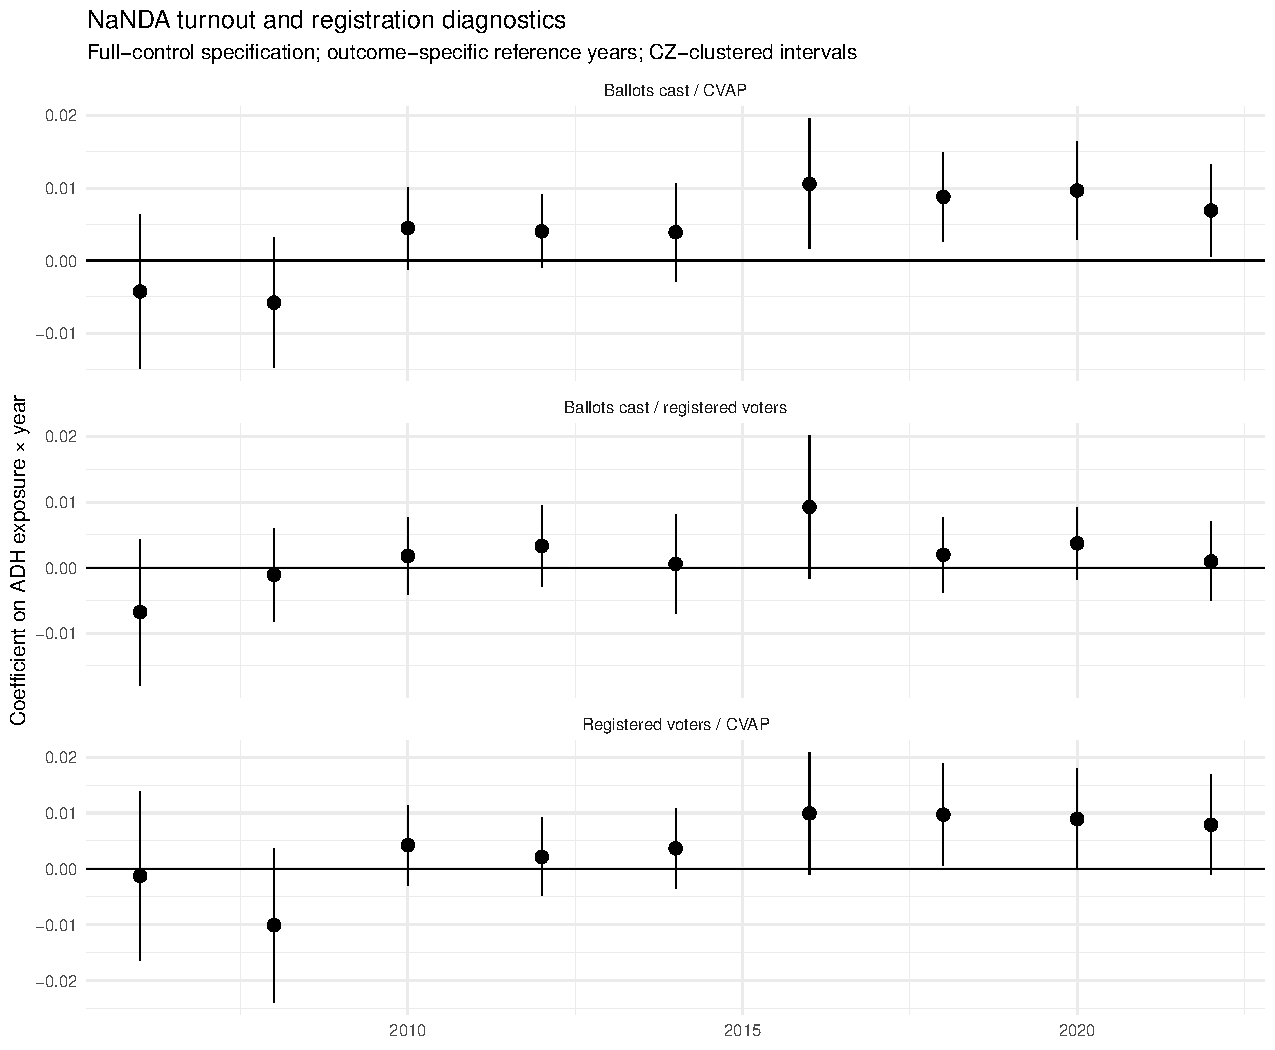
\includegraphics[width=1\linewidth,height=\textheight,keepaspectratio]{../output/figures/fig_nanda_turnout_registration.pdf}

}

\caption{\label{fig-nanda-turnout}NaNDA turnout and registration
outcomes.}

\end{figure}%

\begin{figure}[H]

\centering{

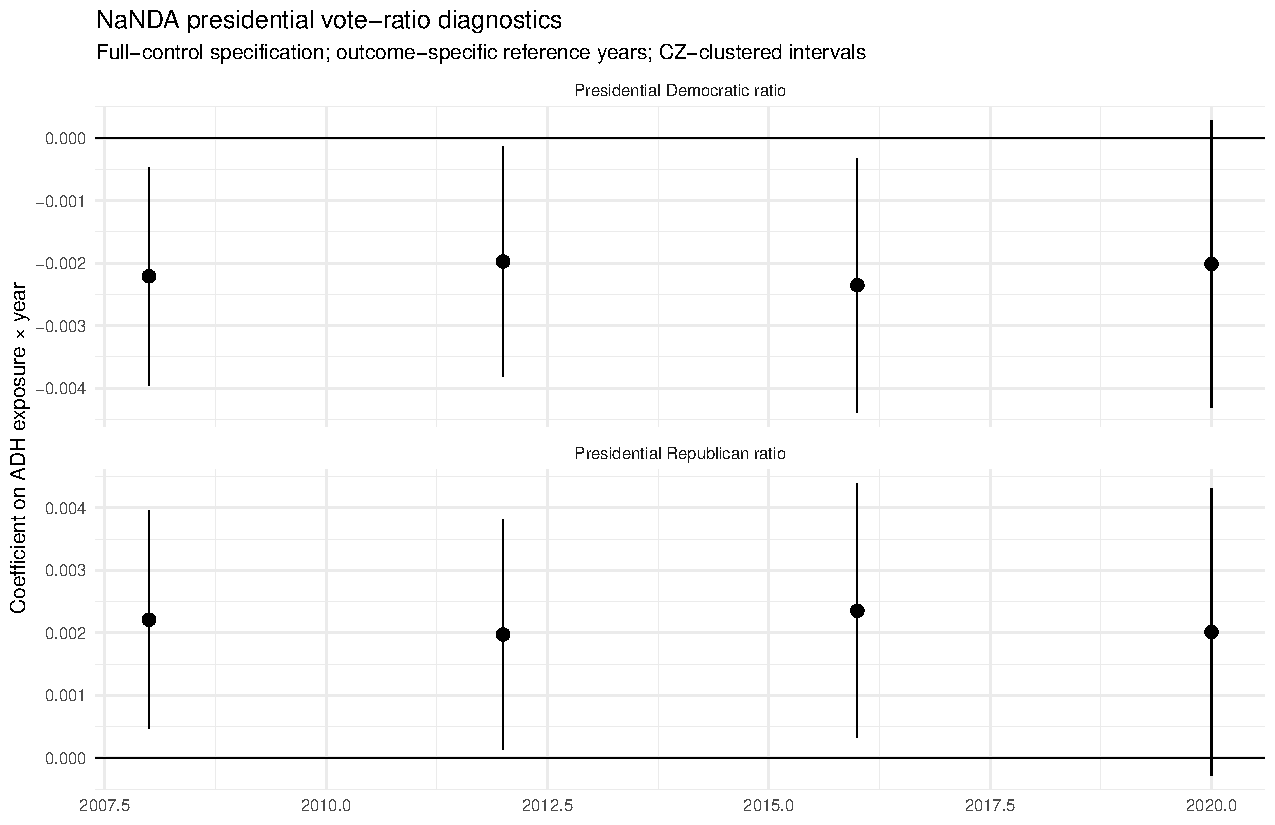
\includegraphics[width=1\linewidth,height=\textheight,keepaspectratio]{../output/figures/fig_nanda_presidential_vote_ratios.pdf}

}

\caption{\label{fig-nanda-vote-ratios}NaNDA presidential vote ratios.}

\end{figure}%

\begin{figure}[H]

\centering{

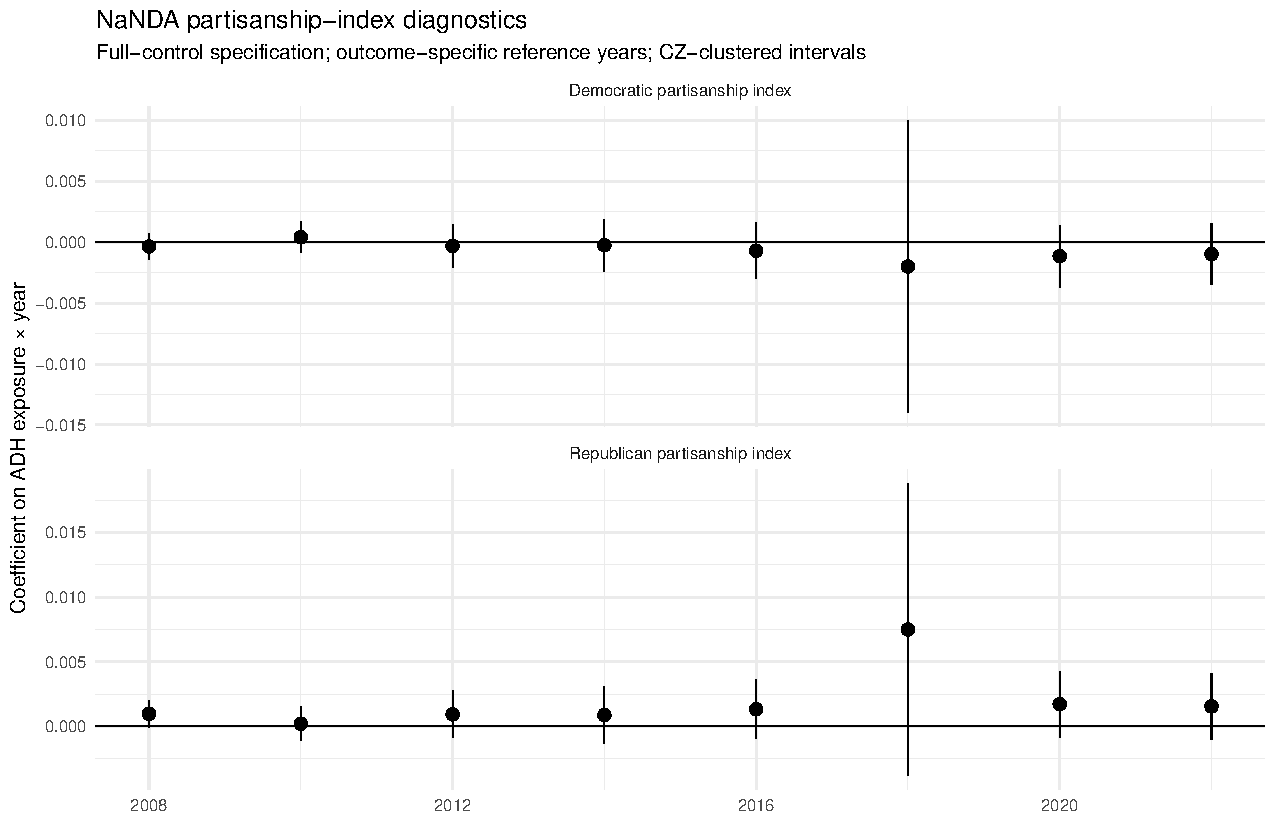
\includegraphics[width=1\linewidth,height=\textheight,keepaspectratio]{../output/figures/fig_nanda_partisanship_indices.pdf}

}

\caption{\label{fig-nanda-partisanship}NaNDA partisanship indices.}

\end{figure}%

{

\begin{longtable}[]{@{}lrrrl@{}}

\caption{\label{tbl-nanda-availability}NaNDA outcome availability by
year.}

\tabularnewline

\toprule\noalign{}
Outcome & Year & Nonmissing CZs & Zero CZs & Available \\
\midrule\noalign{}
\endhead
\bottomrule\noalign{}
\endlastfoot
partisan\_index\_dem & 2004 & 722 & 722 & FALSE \\
partisan\_index\_dem & 2006 & 722 & 0 & TRUE \\
partisan\_index\_dem & 2008 & 722 & 0 & TRUE \\
partisan\_index\_dem & 2010 & 722 & 0 & TRUE \\
partisan\_index\_dem & 2012 & 722 & 0 & TRUE \\
partisan\_index\_dem & 2014 & 722 & 0 & TRUE \\
partisan\_index\_dem & 2016 & 722 & 0 & TRUE \\
partisan\_index\_dem & 2018 & 722 & 253 & TRUE \\
partisan\_index\_dem & 2020 & 722 & 0 & TRUE \\
partisan\_index\_dem & 2022 & 722 & 0 & TRUE \\
partisan\_index\_rep & 2004 & 722 & 722 & FALSE \\
partisan\_index\_rep & 2006 & 722 & 0 & TRUE \\
partisan\_index\_rep & 2008 & 722 & 0 & TRUE \\
partisan\_index\_rep & 2010 & 722 & 0 & TRUE \\
partisan\_index\_rep & 2012 & 722 & 0 & TRUE \\
partisan\_index\_rep & 2014 & 722 & 0 & TRUE \\
partisan\_index\_rep & 2016 & 722 & 0 & TRUE \\
partisan\_index\_rep & 2018 & 722 & 253 & TRUE \\
partisan\_index\_rep & 2020 & 722 & 0 & TRUE \\
partisan\_index\_rep & 2022 & 722 & 0 & TRUE \\
pres\_dem\_ratio & 2004 & 722 & 0 & TRUE \\
pres\_dem\_ratio & 2006 & 0 & 0 & FALSE \\
pres\_dem\_ratio & 2008 & 722 & 0 & TRUE \\
pres\_dem\_ratio & 2010 & 0 & 0 & FALSE \\
pres\_dem\_ratio & 2012 & 722 & 0 & TRUE \\
pres\_dem\_ratio & 2014 & 0 & 0 & FALSE \\
pres\_dem\_ratio & 2016 & 722 & 0 & TRUE \\
pres\_dem\_ratio & 2018 & 0 & 0 & FALSE \\
pres\_dem\_ratio & 2020 & 722 & 0 & TRUE \\
pres\_dem\_ratio & 2022 & 0 & 0 & FALSE \\
pres\_rep\_ratio & 2004 & 722 & 0 & TRUE \\
pres\_rep\_ratio & 2006 & 0 & 0 & FALSE \\
pres\_rep\_ratio & 2008 & 722 & 0 & TRUE \\
pres\_rep\_ratio & 2010 & 0 & 0 & FALSE \\
pres\_rep\_ratio & 2012 & 722 & 0 & TRUE \\
pres\_rep\_ratio & 2014 & 0 & 0 & FALSE \\
pres\_rep\_ratio & 2016 & 722 & 0 & TRUE \\
pres\_rep\_ratio & 2018 & 0 & 0 & FALSE \\
pres\_rep\_ratio & 2020 & 722 & 0 & TRUE \\
pres\_rep\_ratio & 2022 & 0 & 0 & FALSE \\
reg\_voter\_turnout\_pct & 2004 & 717 & 0 & TRUE \\
reg\_voter\_turnout\_pct & 2006 & 661 & 40 & TRUE \\
reg\_voter\_turnout\_pct & 2008 & 670 & 2 & TRUE \\
reg\_voter\_turnout\_pct & 2010 & 703 & 0 & TRUE \\
reg\_voter\_turnout\_pct & 2012 & 700 & 1 & TRUE \\
reg\_voter\_turnout\_pct & 2014 & 702 & 16 & TRUE \\
reg\_voter\_turnout\_pct & 2016 & 699 & 61 & TRUE \\
reg\_voter\_turnout\_pct & 2018 & 701 & 1 & TRUE \\
reg\_voter\_turnout\_pct & 2020 & 702 & 0 & TRUE \\
reg\_voter\_turnout\_pct & 2022 & 704 & 0 & TRUE \\
reg\_voters\_pct & 2004 & 721 & 0 & TRUE \\
reg\_voters\_pct & 2006 & 722 & 50 & TRUE \\
reg\_voters\_pct & 2008 & 721 & 43 & TRUE \\
reg\_voters\_pct & 2010 & 721 & 15 & TRUE \\
reg\_voters\_pct & 2012 & 720 & 16 & TRUE \\
reg\_voters\_pct & 2014 & 721 & 16 & TRUE \\
reg\_voters\_pct & 2016 & 720 & 17 & TRUE \\
reg\_voters\_pct & 2018 & 721 & 16 & TRUE \\
reg\_voters\_pct & 2020 & 720 & 15 & TRUE \\
reg\_voters\_pct & 2022 & 721 & 15 & TRUE \\
voter\_turnout\_pct & 2004 & 722 & 0 & TRUE \\
voter\_turnout\_pct & 2006 & 722 & 62 & TRUE \\
voter\_turnout\_pct & 2008 & 722 & 14 & TRUE \\
voter\_turnout\_pct & 2010 & 722 & 0 & TRUE \\
voter\_turnout\_pct & 2012 & 722 & 2 & TRUE \\
voter\_turnout\_pct & 2014 & 722 & 17 & TRUE \\
voter\_turnout\_pct & 2016 & 722 & 63 & TRUE \\
voter\_turnout\_pct & 2018 & 721 & 1 & TRUE \\
voter\_turnout\_pct & 2020 & 721 & 0 & TRUE \\
voter\_turnout\_pct & 2022 & 721 & 0 & TRUE \\

\end{longtable}

}

\subsection{ADHM 2020 public political-supply
diagnostics}\label{adhm-2020-public-political-supply-diagnostics}

\begin{figure}[H]

\centering{

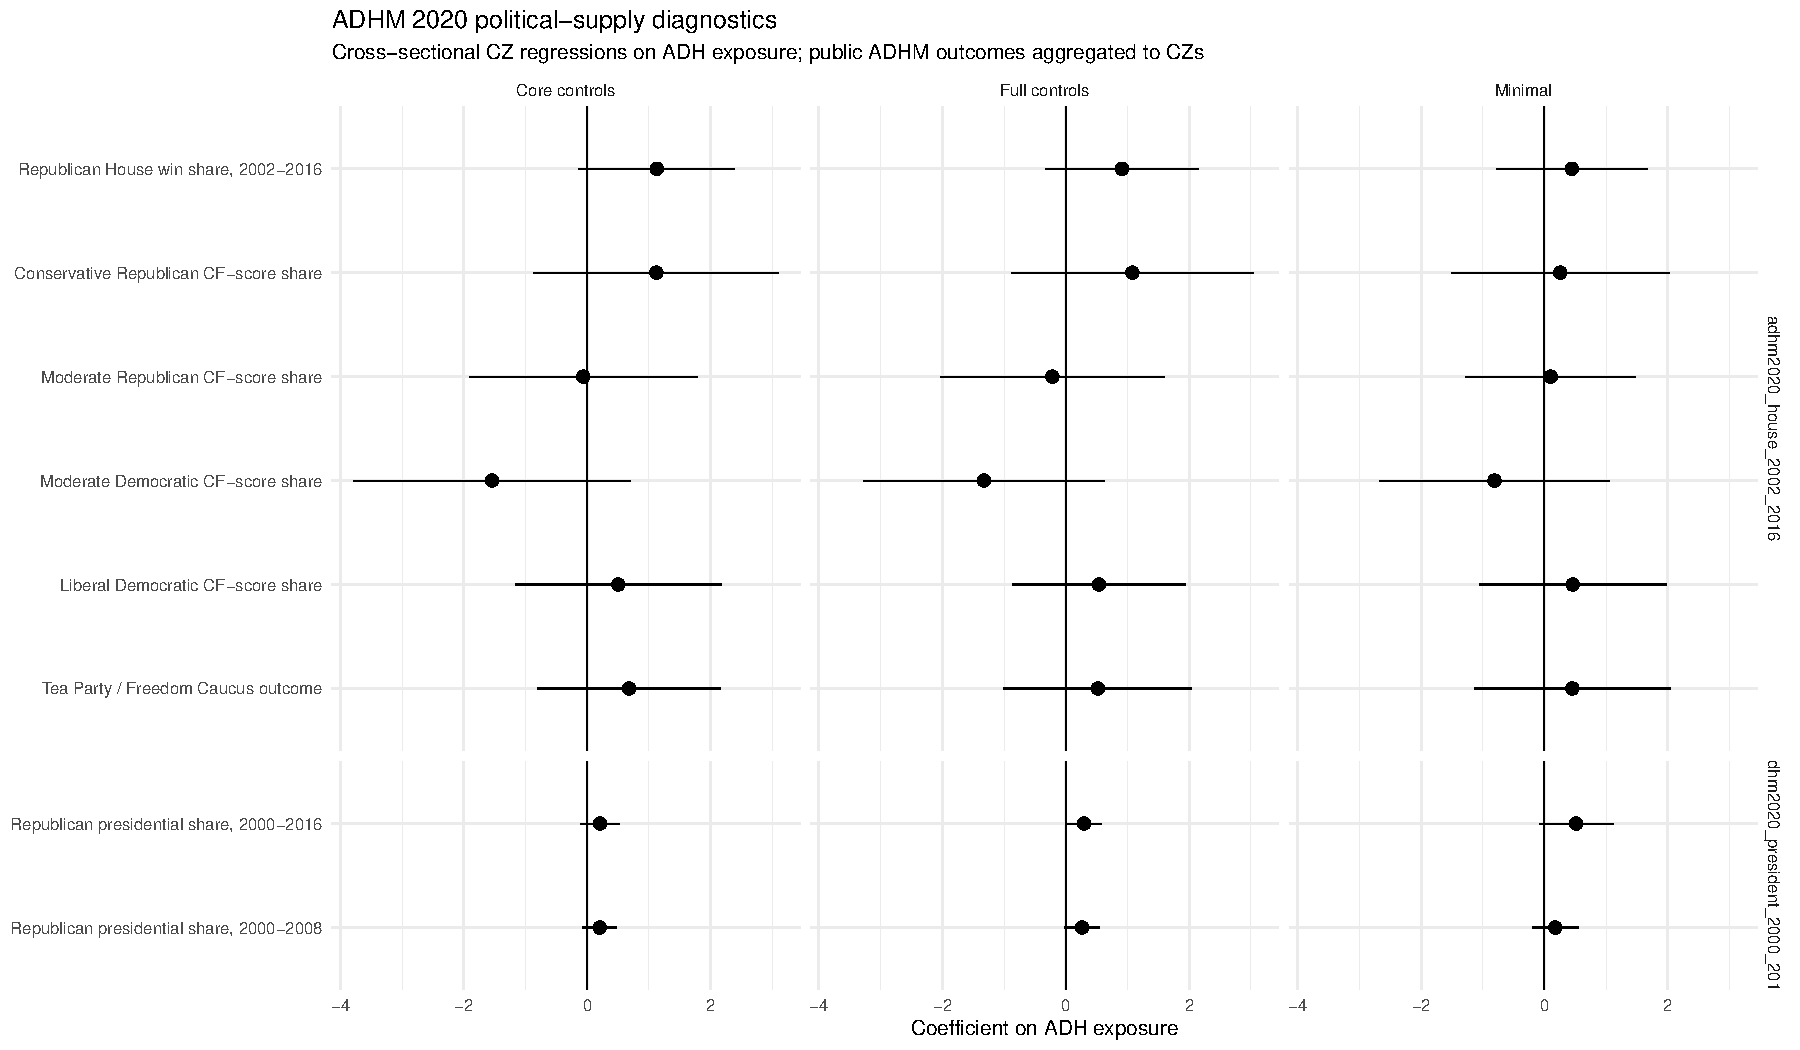
\includegraphics[width=1\linewidth,height=\textheight,keepaspectratio]{../output/figures/fig_adhm2020_mechanism_regressions.pdf}

}

\caption{\label{fig-adhm-mechanisms}ADHM 2020 public political-supply
mechanism regressions.}

\end{figure}%

{

\begin{longtable}[]{@{}
  >{\raggedright\arraybackslash}p{(\linewidth - 10\tabcolsep) * \real{0.4713}}
  >{\raggedright\arraybackslash}p{(\linewidth - 10\tabcolsep) * \real{0.1609}}
  >{\raggedright\arraybackslash}p{(\linewidth - 10\tabcolsep) * \real{0.1034}}
  >{\raggedright\arraybackslash}p{(\linewidth - 10\tabcolsep) * \real{0.1264}}
  >{\raggedright\arraybackslash}p{(\linewidth - 10\tabcolsep) * \real{0.0920}}
  >{\raggedleft\arraybackslash}p{(\linewidth - 10\tabcolsep) * \real{0.0460}}@{}}

\caption{\label{tbl-adhm-mech}ADHM 2020 mechanism regressions.}

\tabularnewline

\toprule\noalign{}
\begin{minipage}[b]{\linewidth}\raggedright
Outcome
\end{minipage} & \begin{minipage}[b]{\linewidth}\raggedright
Spec
\end{minipage} & \begin{minipage}[b]{\linewidth}\raggedright
Estimate
\end{minipage} & \begin{minipage}[b]{\linewidth}\raggedright
Std. error
\end{minipage} & \begin{minipage}[b]{\linewidth}\raggedright
p-value
\end{minipage} & \begin{minipage}[b]{\linewidth}\raggedleft
N
\end{minipage} \\
\midrule\noalign{}
\endhead
\bottomrule\noalign{}
\endlastfoot
Republican House win share, 2002-2016 & Minimal & 0.445 & 0.627 & 0.482
& 722 \\
Republican House win share, 2002-2016 & Core controls & 1.128 & 0.646 &
0.087 & 722 \\
Republican House win share, 2002-2016 & Full controls & 0.911 & 0.632 &
0.156 & 722 \\
Conservative Republican CF-score share & Minimal & 0.256 & 0.901 & 0.778
& 722 \\
Conservative Republican CF-score share & Core controls & 1.122 & 1.013 &
0.274 & 722 \\
Conservative Republican CF-score share & Full controls & 1.080 & 0.999 &
0.285 & 722 \\
Moderate Republican CF-score share & Minimal & 0.103 & 0.703 & 0.884 &
722 \\
Moderate Republican CF-score share & Core controls & -0.063 & 0.944 &
0.947 & 722 \\
Moderate Republican CF-score share & Full controls & -0.216 & 0.925 &
0.816 & 722 \\
Moderate Democratic CF-score share & Minimal & -0.809 & 0.953 & 0.400 &
722 \\
Moderate Democratic CF-score share & Core controls & -1.541 & 1.149 &
0.186 & 722 \\
Moderate Democratic CF-score share & Full controls & -1.326 & 0.995 &
0.189 & 722 \\
Liberal Democratic CF-score share & Minimal & 0.458 & 0.772 & 0.556 &
722 \\
Liberal Democratic CF-score share & Core controls & 0.505 & 0.854 &
0.557 & 722 \\
Liberal Democratic CF-score share & Full controls & 0.538 & 0.714 &
0.455 & 722 \\
Tea Party / Freedom Caucus outcome & Minimal & 0.453 & 0.809 & 0.578 &
722 \\
Tea Party / Freedom Caucus outcome & Core controls & 0.681 & 0.759 &
0.374 & 722 \\
Tea Party / Freedom Caucus outcome & Full controls & 0.520 & 0.778 &
0.508 & 722 \\
Republican presidential share, 2000-2016 & Minimal & 0.514 & 0.307 &
0.101 & 722 \\
Republican presidential share, 2000-2016 & Core controls & 0.210 & 0.160
& 0.196 & 722 \\
Republican presidential share, 2000-2016 & Full controls & 0.296 & 0.148
& 0.052 & 722 \\
Republican presidential share, 2000-2008 & Minimal & 0.176 & 0.192 &
0.362 & 722 \\
Republican presidential share, 2000-2008 & Core controls & 0.204 & 0.142
& 0.159 & 722 \\
Republican presidential share, 2000-2008 & Full controls & 0.265 & 0.145
& 0.075 & 722 \\

\end{longtable}

}

\section{Appendix G: Replication
Notes}\label{appendix-g-replication-notes}

The complete analysis can be regenerated from the project root with:

\begin{Shaded}
\begin{Highlighting}[]
\FunctionTok{source}\NormalTok{(here}\SpecialCharTok{::}\FunctionTok{here}\NormalTok{(}\StringTok{"src"}\NormalTok{, }\StringTok{"run\_pipeline.R"}\NormalTok{))}
\end{Highlighting}
\end{Shaded}

For the final appendix-style crosswalk-sensitivity run:

\begin{Shaded}
\begin{Highlighting}[]
\FunctionTok{Sys.setenv}\NormalTok{(}\AttributeTok{RUN\_CROSSWALK\_SENSITIVITY =} \StringTok{"true"}\NormalTok{)}
\FunctionTok{source}\NormalTok{(here}\SpecialCharTok{::}\FunctionTok{here}\NormalTok{(}\StringTok{"src"}\NormalTok{, }\StringTok{"run\_pipeline.R"}\NormalTok{))}
\end{Highlighting}
\end{Shaded}

The replication-code PDF can be generated from the \texttt{report}
folder with:

\begin{Shaded}
\begin{Highlighting}[]
\FunctionTok{source}\NormalTok{(}\StringTok{"make\_replication\_code\_pdf.R"}\NormalTok{)}
\end{Highlighting}
\end{Shaded}





\end{document}
